\documentclass[a4paper,twoside,11pt]{report}
% Alternative Options:
%	Paper Size: a4paper / a5paper / b5paper / letterpaper / legalpaper / executivepaper
% Duplex: oneside / twoside
% Base Font Size: 10pt / 11pt / 12pt


%% Language %%%%%%%%%%%%%%%%%%%%%%%%%%%%%%%%%%%%%%%%%%%%%%%%%
\usepackage[USenglish]{babel} %francais, polish, spanish, ...
\usepackage[T1]{fontenc}
\usepackage[ansinew]{inputenc}
\usepackage{lmodern} %Type1-font for non-english texts and characters
\usepackage{graphicx} %%For loading graphic files
\usepackage{amsmath}
\usepackage{amsthm}
\usepackage{amsfonts}
\usepackage[style=ieee]{biblatex}
\addbibresource{literature.bib}
\usepackage{csquotes}
\usepackage{blindtext}
\usepackage{parskip}
\usepackage{hyperref}
\usepackage{mathcomp}
\usepackage{float}
\usepackage{geometry}
\usepackage{rotating}
\usepackage{tikz}
\usepackage{wrapfig}
\usepackage{subcaption}
\usepackage{pdfpages}

%% Line Spacing %%%%%%%%%%%%%%%%%%%%%%%%%%%%%%%%%%%%%%%%%%%%%
%\usepackage{setspace}
%\singlespacing        %% 1-spacing (default)
%\onehalfspacing       %% 1,5-spacing
%\doublespacing        %% 2-spacing


%% Other Packages %%%%%%%%%%%%%%%%%%%%%%%%%%%%%%%%%%%%%%%%%%%
%\usepackage{a4wide} %%Smaller margins = more text per page.
\usepackage{fancyhdr} %%Fancy headings
%\usepackage{longtable} %%For tables, that exceed one page

\usepackage{color}

%Definer farger her

\usepackage{titlesec}

\titleformat{\chapter}[display]
{\normalfont\huge\bfseries}{\chaptertitlename\ \thechapter}{20pt}{\Huge}


% this alters "before" spacing (the second length argument) to 0
\titlespacing*{\chapter}{0pt}{0pt}{10pt}
\titlespacing*{\section}{0pt}{0pt}{-4pt}
\titlespacing*{\subsection}{0pt}{0pt}{0pt}
\titlespacing*{\subsubsection}{0pt}{0pt}{0pt}


\definecolor{black}{rgb}{0,0,0}

\parindent 0mm
\setlength{\oddsidemargin}{0mm}
\setlength{\evensidemargin}{0mm}
\setlength{\topmargin}{-20mm}
\setlength{\textwidth}{165mm}
\setlength{\textheight}{260mm}
\parskip 2em


% Farger endres her %%%%%%%%%%%%%%%
% Danner seg noene error meldinger her, de er ikke farlige bare irriterende ut fra det jeg kan se - Erlend %%%%%%%%%%%%%%%%%%%%%
% \hypersetup{
%   pdfauthor={UiA Renewable Student},
%   pdftitle={ENE 228 Designing a fuel cell},
%   colorlinks=true,
  
%   citecolor=black,
%   urlcolor=black,
%   linkcolor=black,
% }

\begin{document}



\pagestyle{empty} %No headings for the first pages.

\begin{titlepage}

\begin{center}

\includegraphics[width=140mm]{DIV./Pics/uia-logo.pdf}

\vspace{1cm}

{\LARGE
\textsc{Designing a fuel cell}}\\

\vspace{0.5cm}

Designing the housing of a single cell PEM fuel cell.

\vspace{4.5cm}

{\bf{Adrian S. Larsen, Erlend Hermansen and Joacim B. Hamre}}

\vspace{4cm}

{\bf{Supervisor}} \\
Peter Hugh Middleton

\vspace{5cm}


\vspace{2cm}

University of Agder, 2019 \\
Faculty of Engineering and Science \\
Department of Engineering Sciences

\end{center}
\end{titlepage}


\clearpage
\pagenumbering{Roman}
\chapter*{Acknowledgements}

    A huge thanks to Peter Hugh Middleton for all the help we received during our project. 

\clearpage
\chapter*{Abstract}

\clearpage
\tableofcontents
\listoffigures
\listoftables
\cleardoublepage %The first chapter should start on an odd page.
\pagestyle{plain} %Now display headings: headings / fancy / ...

\clearpage
\pagenumbering{arabic}

\chapter{Introduction}
    
\section{asd}
\subsection{Background}


The basic principles behind the fuel cell was first demonstrated by Humphry Davy in 1801, and in 1839 William Grove created the first fuel cell. Grove called his invention a gas battery. In 1889, Charles Langer and Ludvig Mond gave the technology the name fuel cell. After this there is a long gap in history of little development on the fuel cell until the 1950s when General Electric created the first Proton-exchange membrane (PEM) fuel cell. Since the 1950s fuel cells have been used to power a lot of different vehicles and other technology. Some exampels of uses are in NASA space missions in 1960s, in submarines by the US Navy in 1980s and in cars by Honda in 2008.

As we are phasing out fossil fuels as energy resource in the transporting sector there have been created a need for other more environmental friendly technologies to take over. In this vacuum fuel cell technology have blossomed. Especially in fields where battery storage is an inefficient way of storing energy.

\subsection{Outline}

In this project we are going to study the PEM fuel cell to get a better understanding of the concept of fuel cells. During our project we are going to design and test a single cell PEM fuel cell. Using Solidworks to create a 3D model of the housing and 3D printers to make the housing.

After printing and assembling the Membrane Electrode Assemblies (MEA), and the housing to a complete single cell fuel cell, we are going to test the voltage and power output of the fuel cell. We are also going to look at the difference in performance of the fuel cell with and without the nickle foam gas diffusion layer.


%As the world faces two big problems, global warming and resource shortage the need for renewable energy sources are increasing. Exactly because of this, the fuel cell has a great appeal as it generates electricity with very low pollution with the fuels consisting of hydrogen and oxygen. This can with optimized technology be a very good alternative to fossil fuels. 

\chapter{Theory on PEM fuel cell}
    \section{Basic Principles}
The purpose of the fuel cell is to produce an electrical current that can be used to do work like powering a motor or illuminating a light bulb. A chemical reaction inside the fuel cell converts electrochemical energy into electrical energy. A reaction occurs between hydrogen fuel and oxygen or another oxidizing agent creating a DC current. Two electrodes, anode and cathode, allows for a reduction-oxidation process to occur through the catalyst and external electric circuit. 

At the anode, which is the negative electrode, a oxidation process will occur with the following half cell reaction
\begin{equation}
    2H_2 \rightleftharpoons 4H^++ 4e^-
\end{equation}

While at the cathode, which is the positive electrode, the reduction process will occur with the following half cell reaction
\begin{equation}
    O_2 +4H^+ + 4e^- \rightleftharpoons 2H_2O
\end{equation}

This will give us a overall reaction as following
\begin{equation}
    2H_2 + O_2 \rightleftharpoons 2H_2O
\end{equation}


Pressurized hydrogen $(H_2)$ will enter at the anode where it will come in contact with the catalyst causing the $H_2$ molecule to split into two $H^+$ ions and two electrons. At the opposite side, oxygen gas $(O_2)$ will enter at the cathode and form two oxygen atoms with strong negative charges. This negative charge will attract the $H^+$ ions to pass through the membrane, while the electrons are blocked from passing through the membrane and forced through an external circuit. On the other side the $H^+$ ions will recombine with an oxygen atom and two electrons from the external circuit to create a water molecules $(H_2O)$.


Since the fuel cell creates electricity from a chemical reaction, rather than combustion, it will not be a subject to thermodynamic laws like "Carnot Limit" and will be more efficient in transforming energy from fuels to usable electrical energy. To further increase the efficiency of the fuel cell, the waste heat can be harnessed. However activation energy needs to be supplied to cross the thermodynamic barrier.

To cross this thermodynamic barrier a  catalyst can be applied to the electrodes and the membrane to increase the kinetics of the reaction which will determine how fast the reactions occurs. We can also increase the surface area of the electrodes, as well as raise the temperature. 

\begin{figure}[ht]
    \centering
    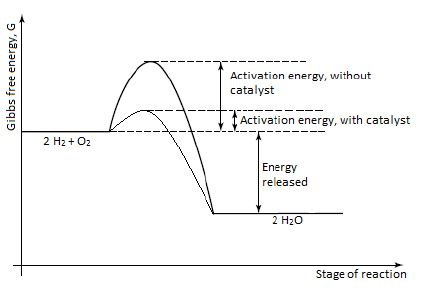
\includegraphics[width=0.9\textwidth]{DIV./Bilder/activation.jpg}
    \caption{Activation energy diagram}
    \label{fig:Activation}
\end{figure}

The driving force of these chemical reactions is the Gibbs free energy and change in Gibbs free energy lets us calculate the ideal no loss voltage for a single cell to 1.23 V with the following equation
\begin{equation}
    \Delta G = zFE^0
\end{equation}

Where
\begin{center}
    $\Delta$G = Change in Gibbs free energy under standard conditions [$J/Mol$] \\
    z = Number of electrons [-] \\
    F = Faradays constant [$C/Mol$] \\
    $E^0$ = EMF under standard conditions [$V$]
\end{center}

In reality a fuel cell will have lower voltage because of losses. Some losses are caused by fuel crossover, internal current losses, ohmic losses, and mass transport or concentration losses. The Cell voltage output is given by the following
\begin{equation}
    V_{cell} = E_{ocv} - \Delta V_{activasion} - \Delta V_{ohmic} - \Delta V_{mass}
\end{equation}

$E_{ocv}$ is given by the thermodynamic EMF

\begin{equation}
    E_{ocv} = - \frac{\Delta G}{zF}
\end{equation}


\begin{figure}[ht]
    \centering
    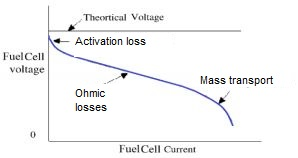
\includegraphics[width=0.9\textwidth]{DIV./Bilder/Assembly/losses.jpg}
    \caption{Fuel cell current-voltage characteristic}
    \label{fig:Fuel cell current-voltage characteristic}
\end{figure}

The efficiency of the PEMFC is calculated using the following equation
\begin{equation}
    \eta =  \frac{E_1}{E^0}
\end{equation}

Where
\begin{center}
$\eta$ = the efficiency of the fuel cell \\
$E_1$ = Measured fuel cell voltage \\
$E^0$ = No loss voltage    
\end{center}

Another challenge with the PEMFC is water balance. In each cell water is being formed and depending on operating conditions and the load, the fuel cell can both be flooded and dried out. If the fuel cell is flooded it can prevent reactant diffusion to the catalyst by flooding the electrodes. A dried-out fuel cell will decrease the electrolytes proton conductivity, which will increase the cell resistance and decrease the efficiency of the fuel cell. It is important that the membrane has just the right moisture level without flooding or drying it out to get the best possible efficiency.

.....Gas diffusion, for å spre gassen mest mulig slik at man får flest mulig reaksjoner.....

\section{Components}

\begin{figure}[h]
    \centering
    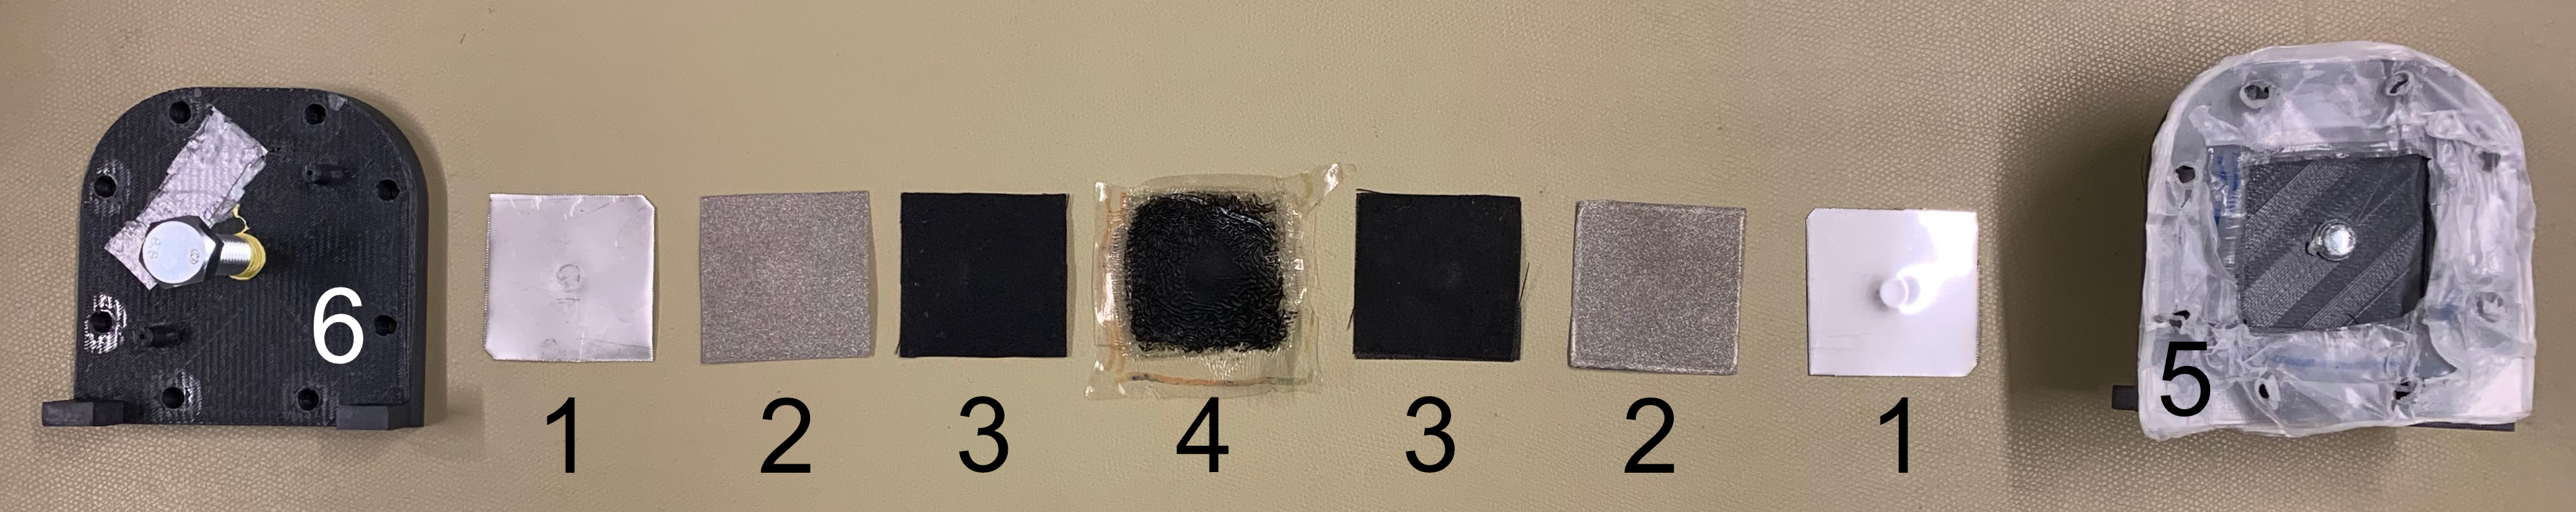
\includegraphics[width=\textwidth]{DIV./Bilder/layout.jpg}
    \caption{Components in PEM fuel cell}
    \label{fig:Components}
\end{figure}

\subsection{Anode and cathode}
Hydrogen will enter at the negative electrode of the PEMFC called the anode. The job of the anode is to conduct electrons that are freed from the hydrogen molecules to be used in an external circuit. Our anode is a carbon paper with a thin layer of catalyst on the side facing the membrane.

Oxygen will enter at the positive electrode of the PEMFC called the cathode. Just as our anode, the cathode is a carbon paper with a thin layer of catalyst on the side facing the membrane. The job of the cathode is to conduct electrons back from the external circuit to the catalyst, here they will recombine with $H^+$ ions and oxygen to form water. The anode and cathode can be seen on figure \ref{fig:Components}

\begin{figure}[h]
    \centering
    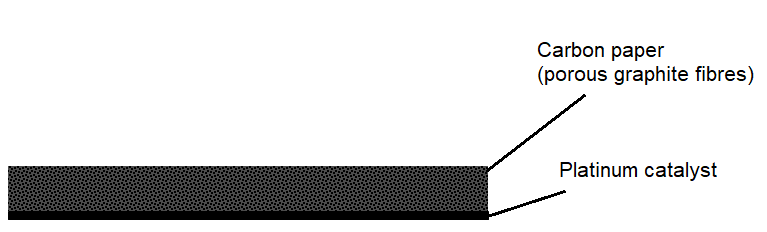
\includegraphics[width=0.6\textwidth]{DIV./Bilder/carbonpaper.png}
    \caption{Electrodes - Carbon paper}
    \label{fig:Electrodes}
\end{figure}

\subsection{Electrolyte}
Ath the heart of the fuel cell sits an electrolyte  and in a PEMFC this is a proton exchange membrane. This membrane allows $H^+$ ions to pass through unhindered while electrons and other substances are blocked from passing through. The membrane is made up by a specially treated material, so that it only conducts positively charged ions. The electrolyte in a  PEMFC is usually is a thin transparent proton exchange membrane called Membrane Electrolyte Nafion (MEA) with a thickness of about \( 50\ \mu \)m


\begin{figure}[h]
    \centering
    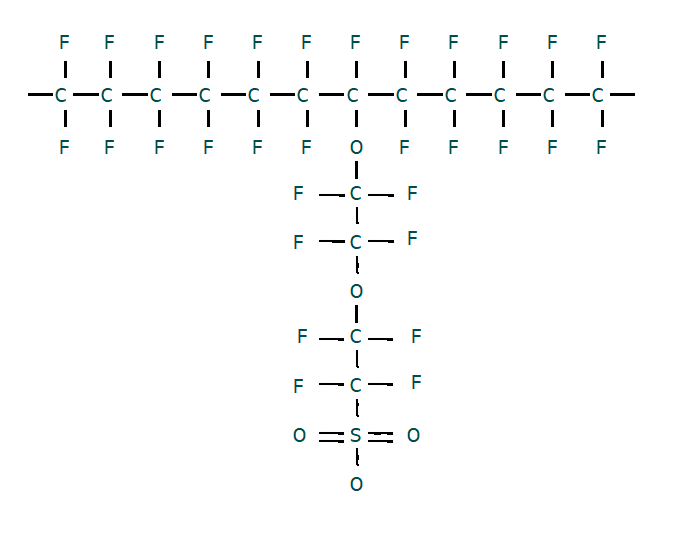
\includegraphics[width=0.7\textwidth]{DIV./Bilder/polymersheet.png}
    \caption{Sulphonated flourethylene Nafion \cite{PemLectue}}
    \label{fig:Nafion}
\end{figure}

\subsection{Catalyst}
The catalyst in our PEMFC is a mix of carbon-platinum and isopropyl alcohol (IPA) painted onto both sides of our electrolyte and also onto both of the carbon electrodes.

This is made up of a special material that facilitates the reaction of oxygen and hydrogen. It is most commonly made up by a very thin coat of platinum nanoparticles onto carbon paper or a piece of cloth. To expose the hydrogen and oxygen as much as possible to the platinum the catalyst will be rough and porous. 

\begin{wrapfigure}{r}{0.5\textwidth}
  \begin{center}
    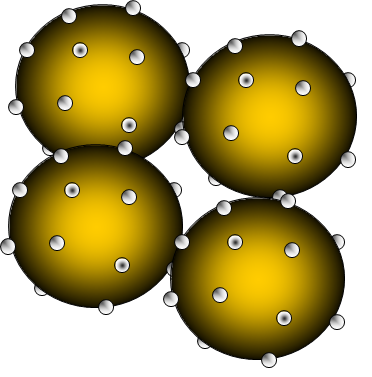
\includegraphics[width=0.3\textwidth]{DIV./Bilder/Catalyst.png}
  \end{center}
  \caption{Small platinum particles on carbon particles \cite{PemLectue}}
\end{wrapfigure}
    

\chapter{Methods in... }
    \section{Work plan}

To spend our time as efficient as possible we decided to make a plan of how much progress was to be done on the fuel cell the following weeks. The work plan gave us deadlines for what was to be done and gave us an easy way to keep track of that was to be done each week.

\begin{center}
    \begin{table}[h]
        \centering
        \begin{tabular}{|c|c|}
        \hline
        Week & Time \\
        \hline
        1 & Concept brainstorming and sketching  \\ 
        \hline
        2 & Creating modulation in Solidworks \\
        \hline
        3 & 3D printing housing part \\
        \hline
        4 & Assembling and testing \\ 
        \hline
     \end{tabular}
     \caption{Plan of progress}
     \label{tab:Workplan}
    \end{table}
\end{center}



\section{Modulation of housing parts}

We used the program Solidworks to modulate the fuel cell housing parts. The housing parts dimensions were determined on the bases of the fuel cell chamber as we needed enough space between the chamber and the outer dimensions of the housing parts for the sealant to have enough space to seal properly. The maximum parameter we were given for the fuel cell itself was 50x50mm therefor the chamber dimensions were set for us. We decided that 25mm spacing between the chamber and the outer dimensions of the fuel cell would be enough space to seal the two parts together. Thereby making the fuel cells outer dimensions 100x100mm. To not use excessive amounts of filament and time while 3D printing, and still make the two housing parts strong enough to withstand wear and tear, we decided that a thickness of 10mm of would be sufficient. As the fuel cell chamber needed a volume that would hold two metal plates with a thickness
 of.. and the fuel cell itself, the depth in each part was sett to be 2mm. Making the total dimensions of the fuel cell housing to be 100x100x20mm with a chamber of 50x50x4mm.


To pin the two housing parts together we decided to use M6 bolts. There were made two holes on each side of the housing parts, making a total of eight bolt holes per part. To easily fit the M6 bolts we made the bolthole diameter 6,5mm as the M6 bolts have a diameter of 6mm. The middle bolthole was modeled and 3D printed with a diameter of 10mm but was threaded to fit an M12 bolt after the parts were printed. 

\section{The 3D printer}

\subsection{Ultimaker 2 Go/2+}

The printers used in this project are the Ultimaker 2 Go and Ultimaker 2+. The Ultimaker 2 Go is a small printer, able to print builds up to 120 x 120 x 115 mm. For this project this printer was used to print prototypes and to learn how to use the 3D printers. The reason for this is the high printig speed and high availability at the lab. Due to safety margins on the printer it was not possible for us to print the full scale housing on this printer. The fact sheet for the printer can be found in appendix C.

The Ulitmake 2+ has the ability to print builds up to 223 x 223 x 205 mm. This was the printer used to print the final housing parts for the PEM fuel cell. 

\subsection{Filament}

The filament we used is Polylactic acid (PLA) plastic. The filament used has a printing temperature of 180-210 \textdegree C and a melting point at 145-160 \textdegree C. The technical sheet for the fillament can be found in appendix D.

\subsection{Ultimaker Cura}

To print the 3D model created in Solidworks the slicer program Ultimaker Cura was used. The slicer program turns the 3D model into several "slices" which the printer then can print. Ultimaker Cura also generated the necessary amount of support structure to pint the housing parts. 

\section{Printing the model}

\subsection{Printing of draft housing} 

After completing the modeling in Solidworks, we decided to print scaled down version of one side of the housing. We scaled the oxygen side of the housing down to 40\% of the original size and printed it. Our goal by printing a small scale model was to look for design errors we could not find on the computer model. Printing the draft was also a good way to learn how the 3D printers worked as none of us had used them before.

The first draft print did not go as planed. After about half an hour the printer failed and we had to abort the printing process. The results of the first draft print can be seen on the picture below, figure \ref{fig:Draft1}.


\begin{figure}[ht]
    \centering
    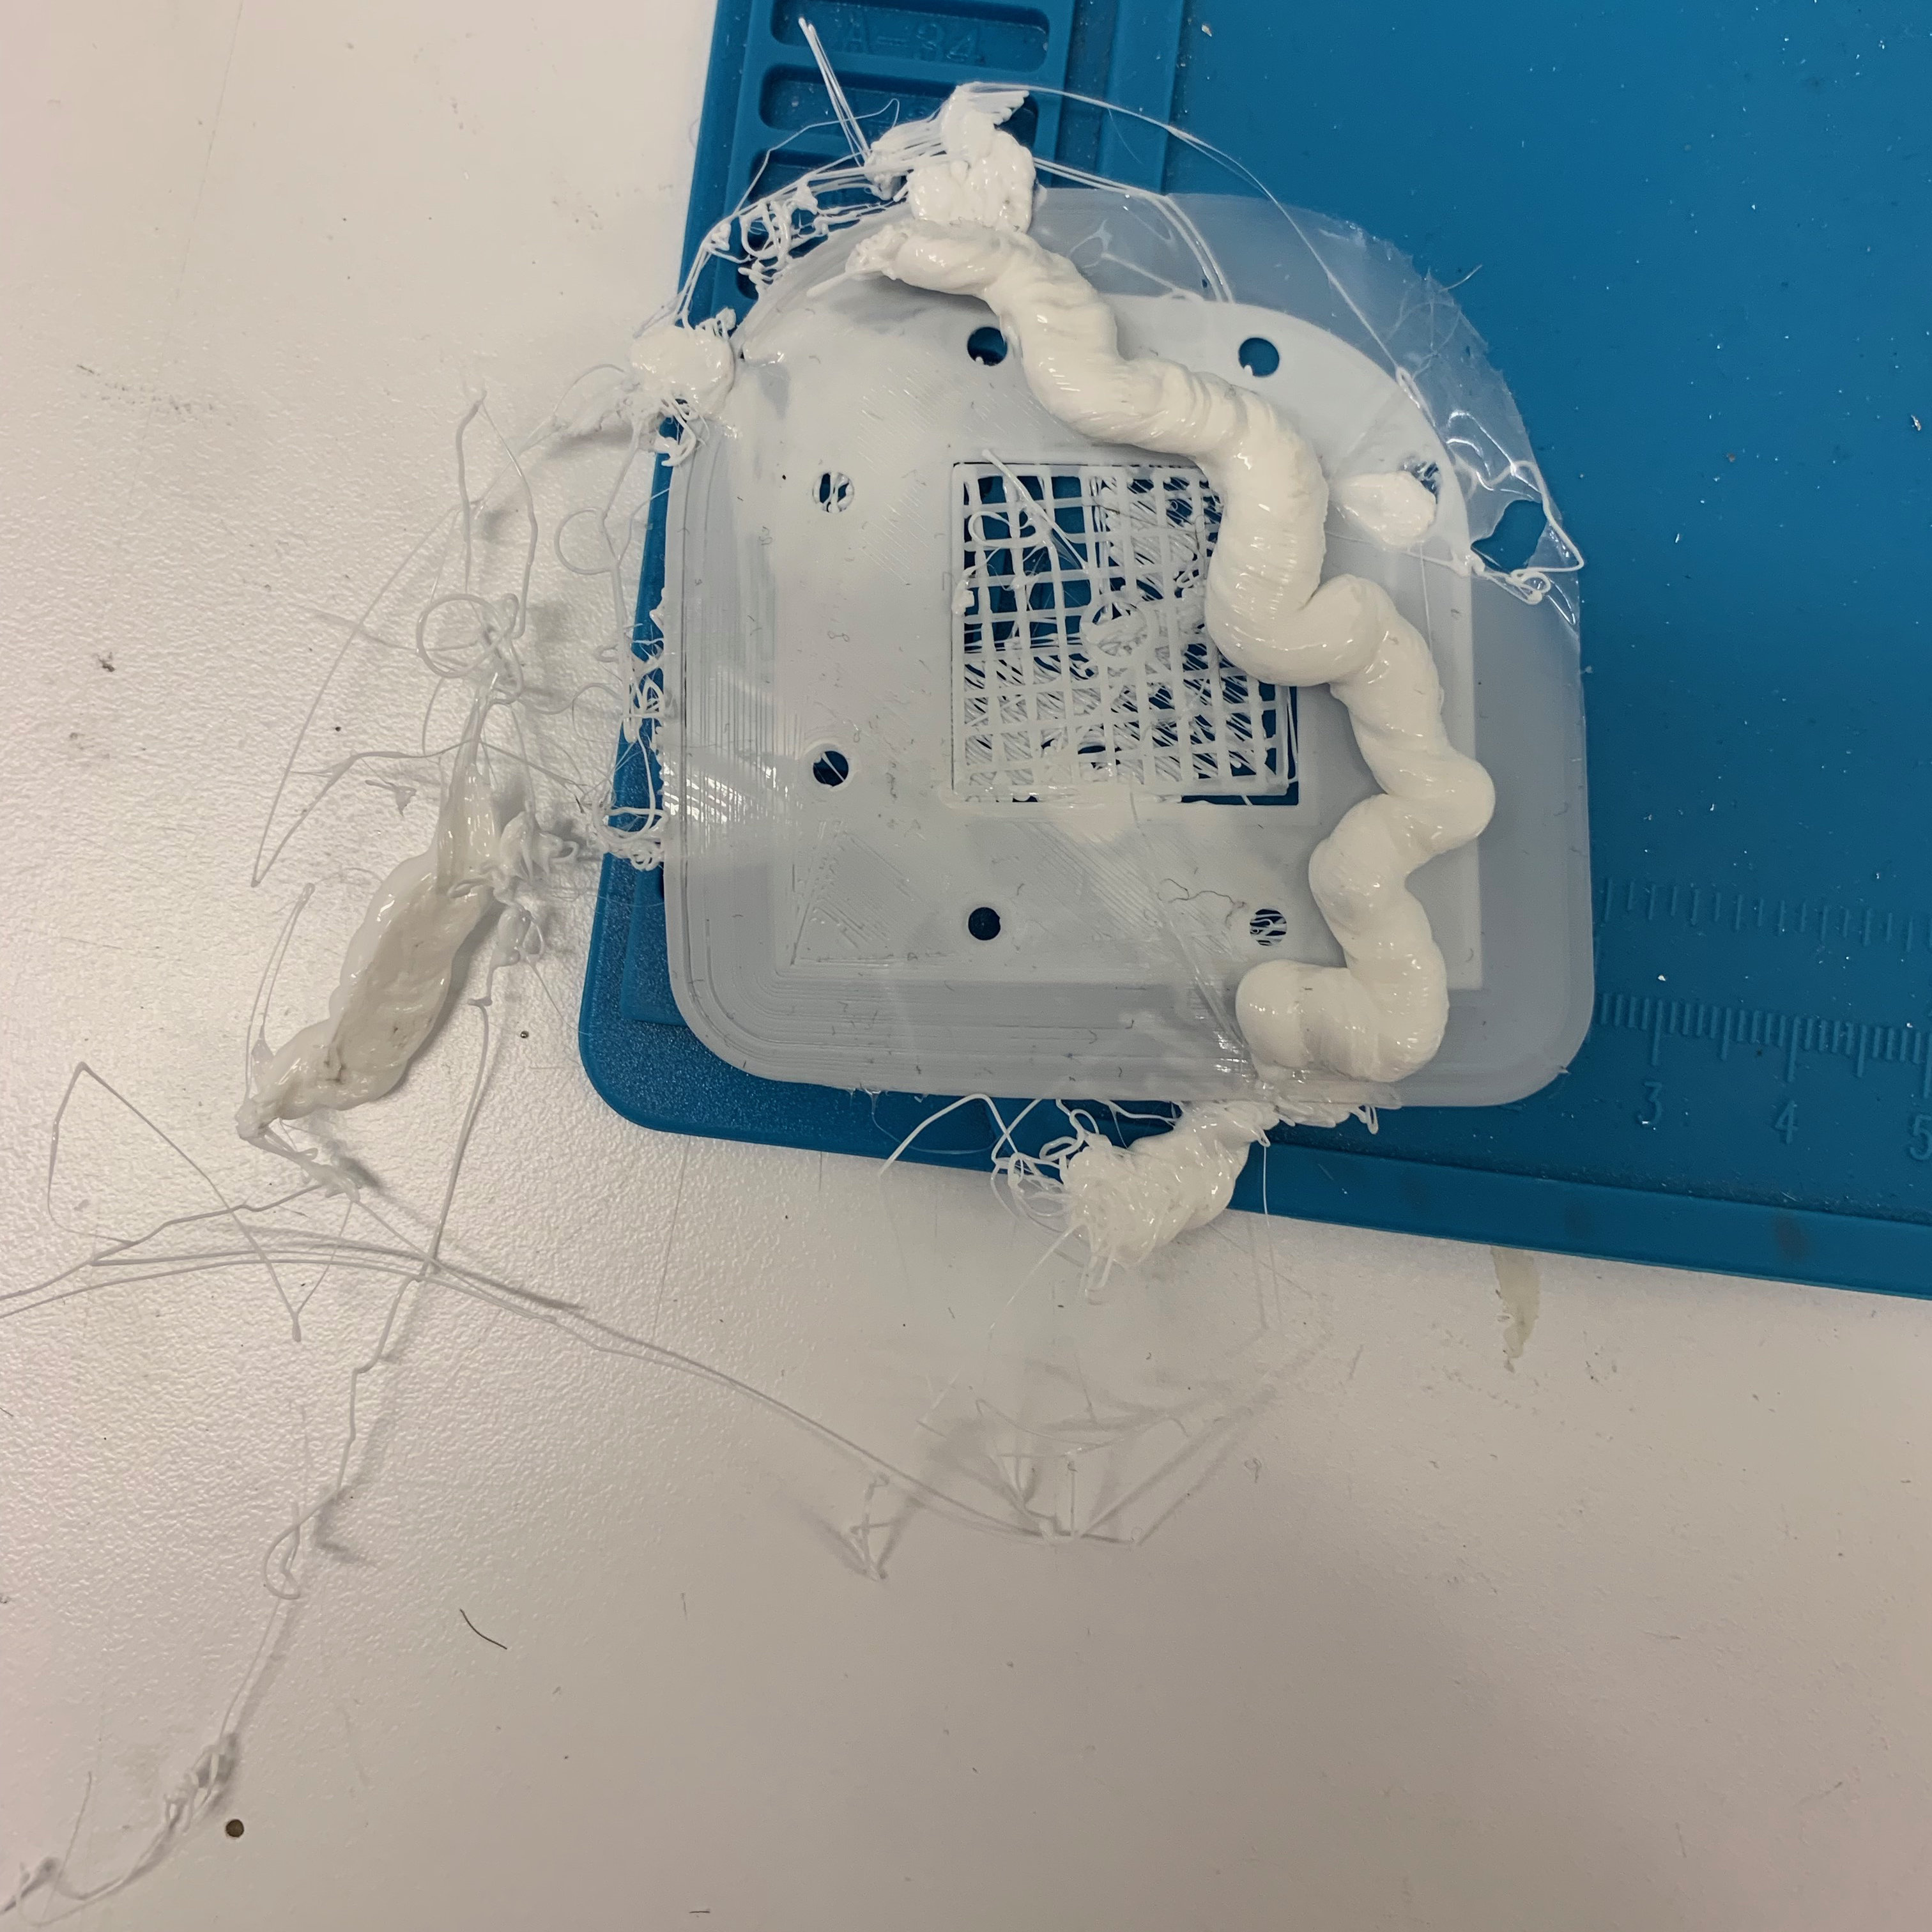
\includegraphics[width=0.40\textwidth]{DIV./Bilder/Draft1.jpg}
    \caption{Picture of the first draft print}
    \label{fig:Draft1}
\end{figure}

As the first draft print failed, we started to look for errors in the printing file and errors on the 3D printer. What we found was that the model had moved on the building plate during the printing. To fix this problem we covered the top of the building plate in masking tape to create more friction. We also made a new printing file just to be on the safe side. 

After an hour of printing the small scale model was complete. This time the result was good. We got a great look at how our design was going to look like. We did not find anything that we needed to change before printing the full scale model.

\subsection{Printing the housing}

\subsubsection{Scaled Prototype}

As the 40\% scale housing looked fine we proceeded by creating the printing file for the full size housing. In order to use the least amount of time possible on waiting for 3D printers to become available we decided to print both the hydrogen and oxygen side at the same time. 

\subsubsection{First print}

After 24 hours of printing we discovered that the print had failed. The tape had separated from the building plate. As a result of this the sides of the housing had begun to curve and deform. There was no reason til continue the print, and we aborted the print. The building plate was cleaned and the print was scraped. 

\begin{figure}[ht]
    \centering
    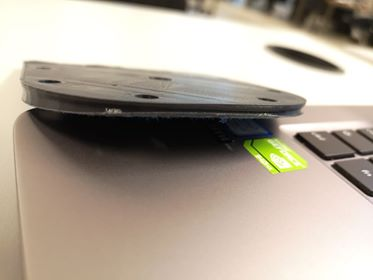
\includegraphics[width=0.6\textwidth]{DIV./Bilder/Firstprint.jpg}
    \caption{Picture of the first print}
    \label{fig:Print1}
\end{figure}

\subsubsection{Final print}

After the print failed we looked for errors. Our conclusions was that due to the large surface area of the building plate being printed on the amount of heat had affected the tape. We decided to print each side of the fuel cell by themselves and build some support structure under the housing part. By building the support structure we hoped it let some of the heat dissipate. Figure \ref{fig:Housingprint} is taken during the printing of the oxygen side of the housing and shows the support structure printed under the housing part.

\begin{figure}[ht]
    \centering
    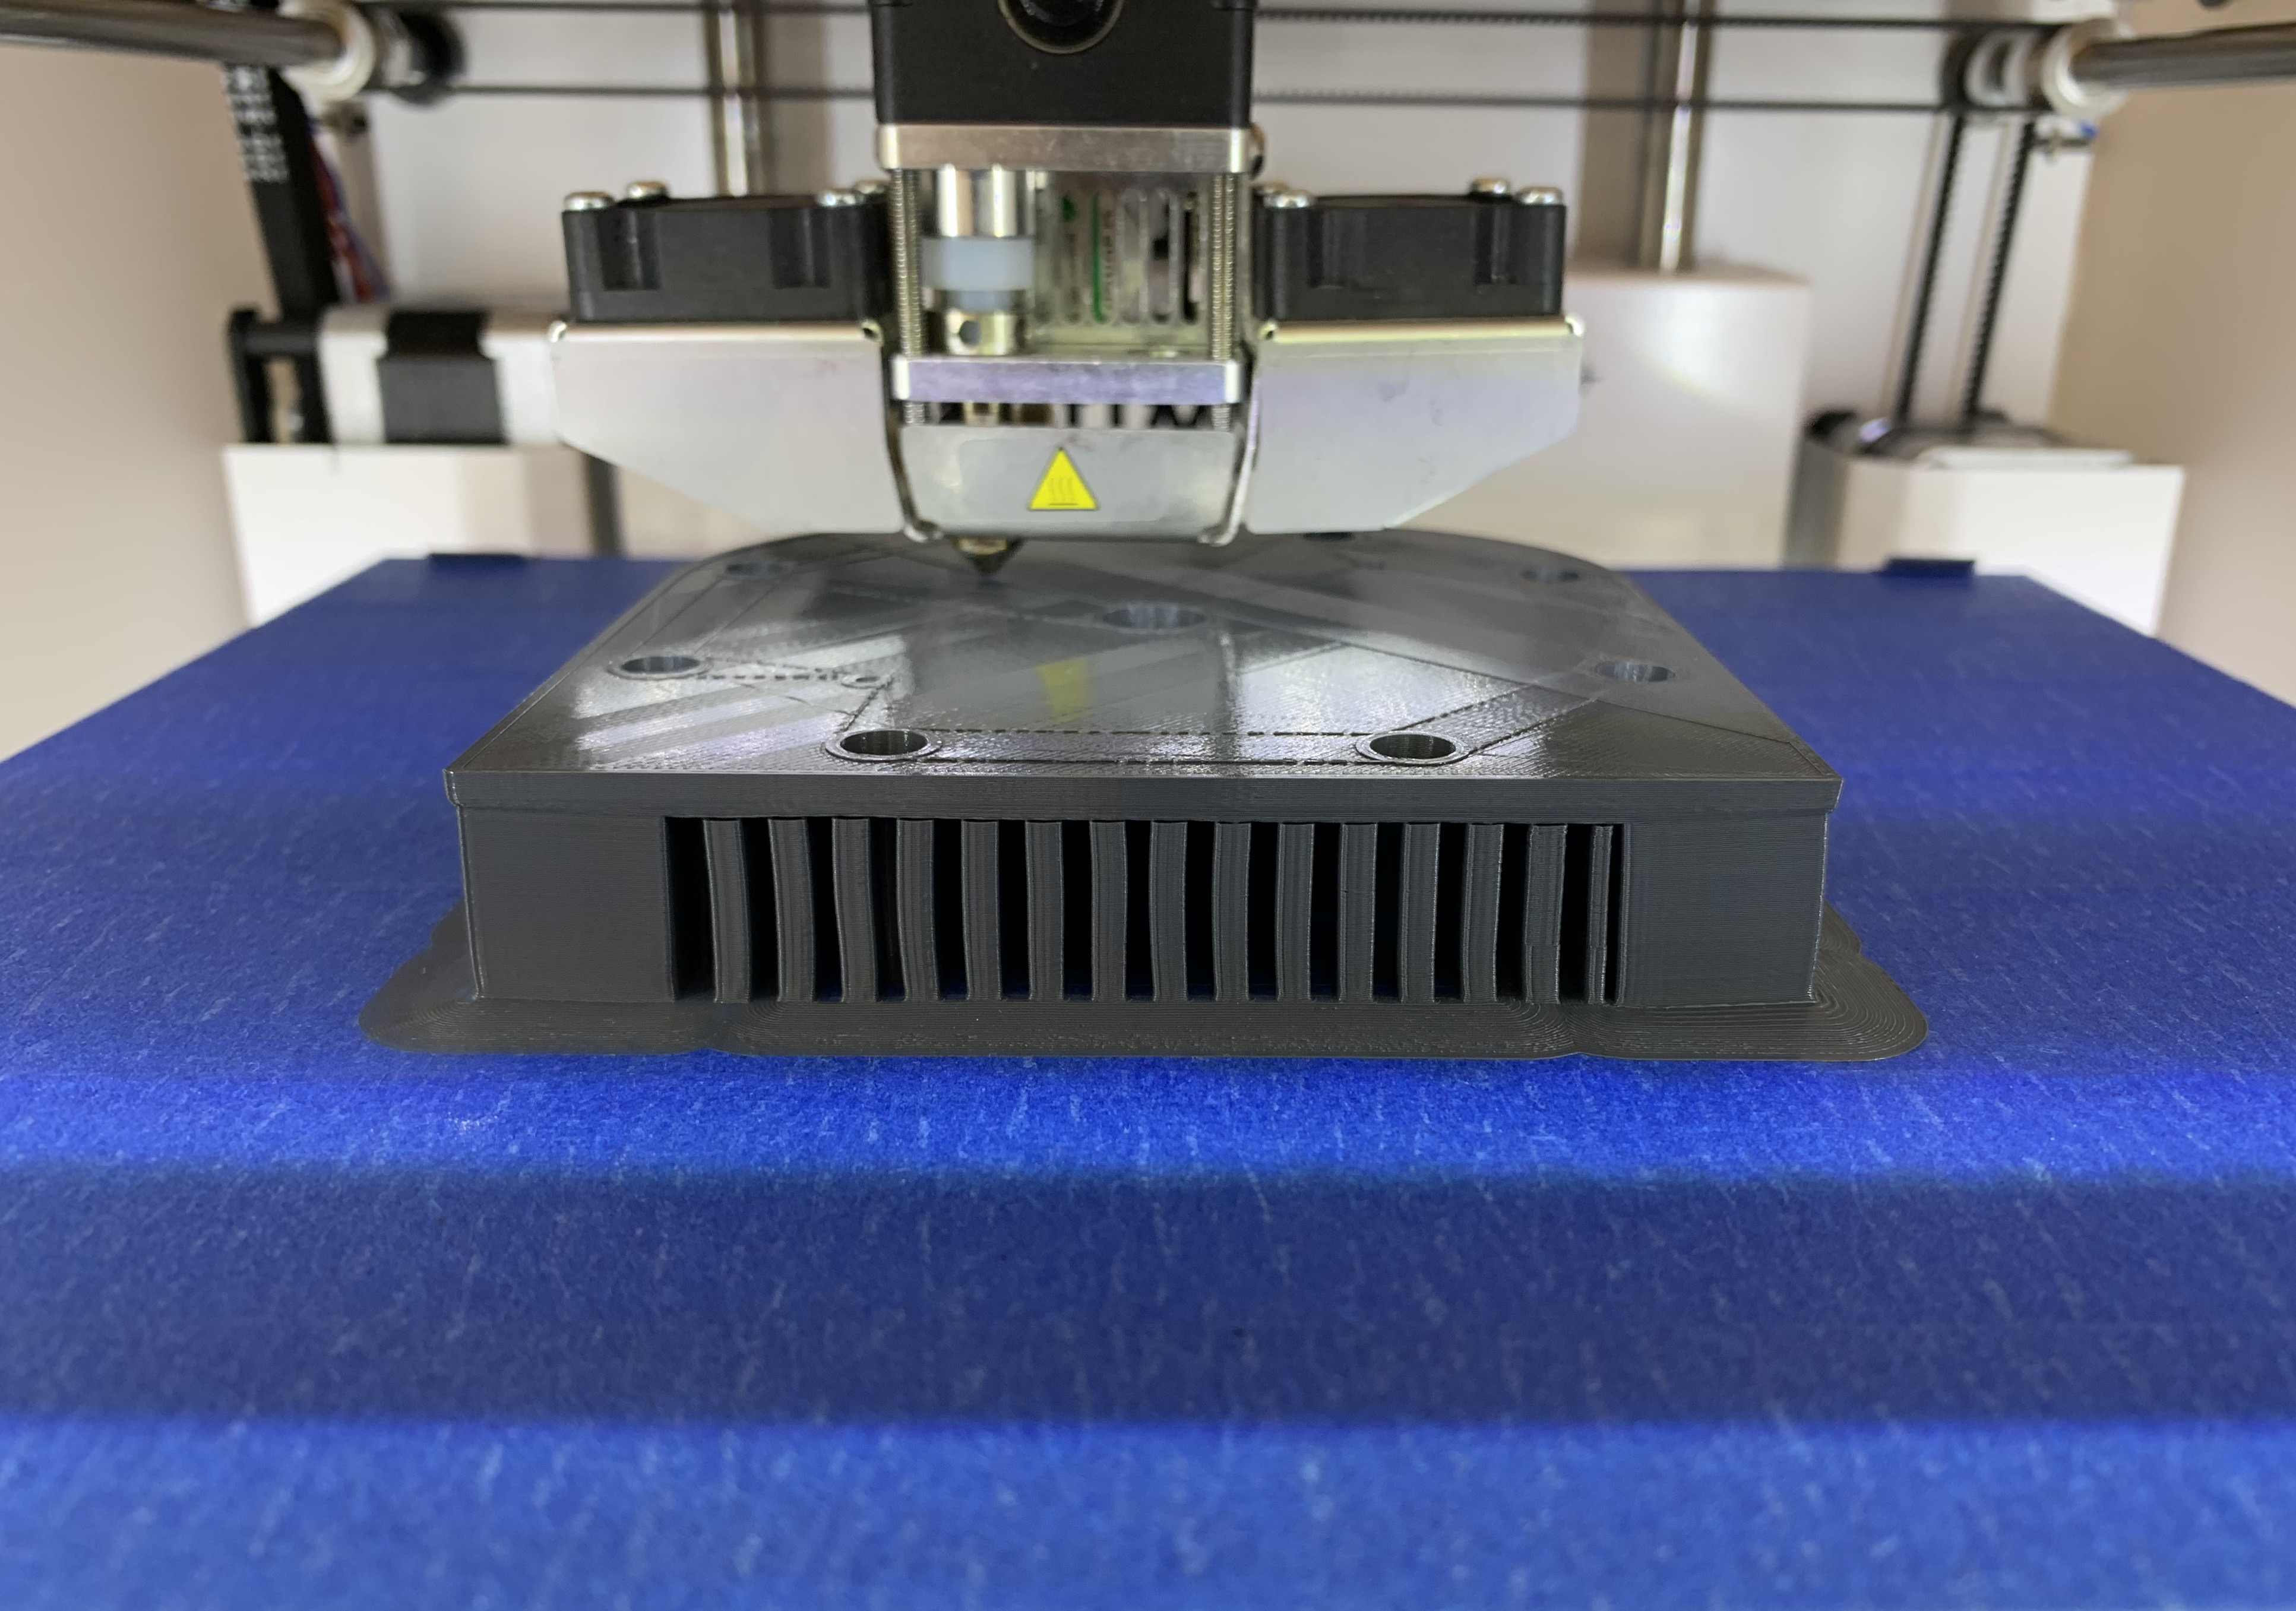
\includegraphics[width=0.6\textwidth]{DIV./Bilder/FinalPrint.jpg}
    \caption{Oxygen side being printed}
    \label{fig:Housingprint}
\end{figure}

\section{Assembling the fuel cell}

\subsection{Assembly with nickel foam gas diffusion layer}

When assembling the fuel cell we started by putting a double layer of Parafilm, PM-992, around the edges PEMFC housing to create a gas seal to make sure that no gas could escape. We also added a metal plate to create electrodes, for easy current collection. To allow the gas to get in front of the metal plate the corners blocking the input and output of the gases was cut away. As you can see on figure \ref{fig:GasSealMetal}.

\begin{figure}[ht]
    \centering
    \begin{subfigure}[b]{0.3\textwidth}
        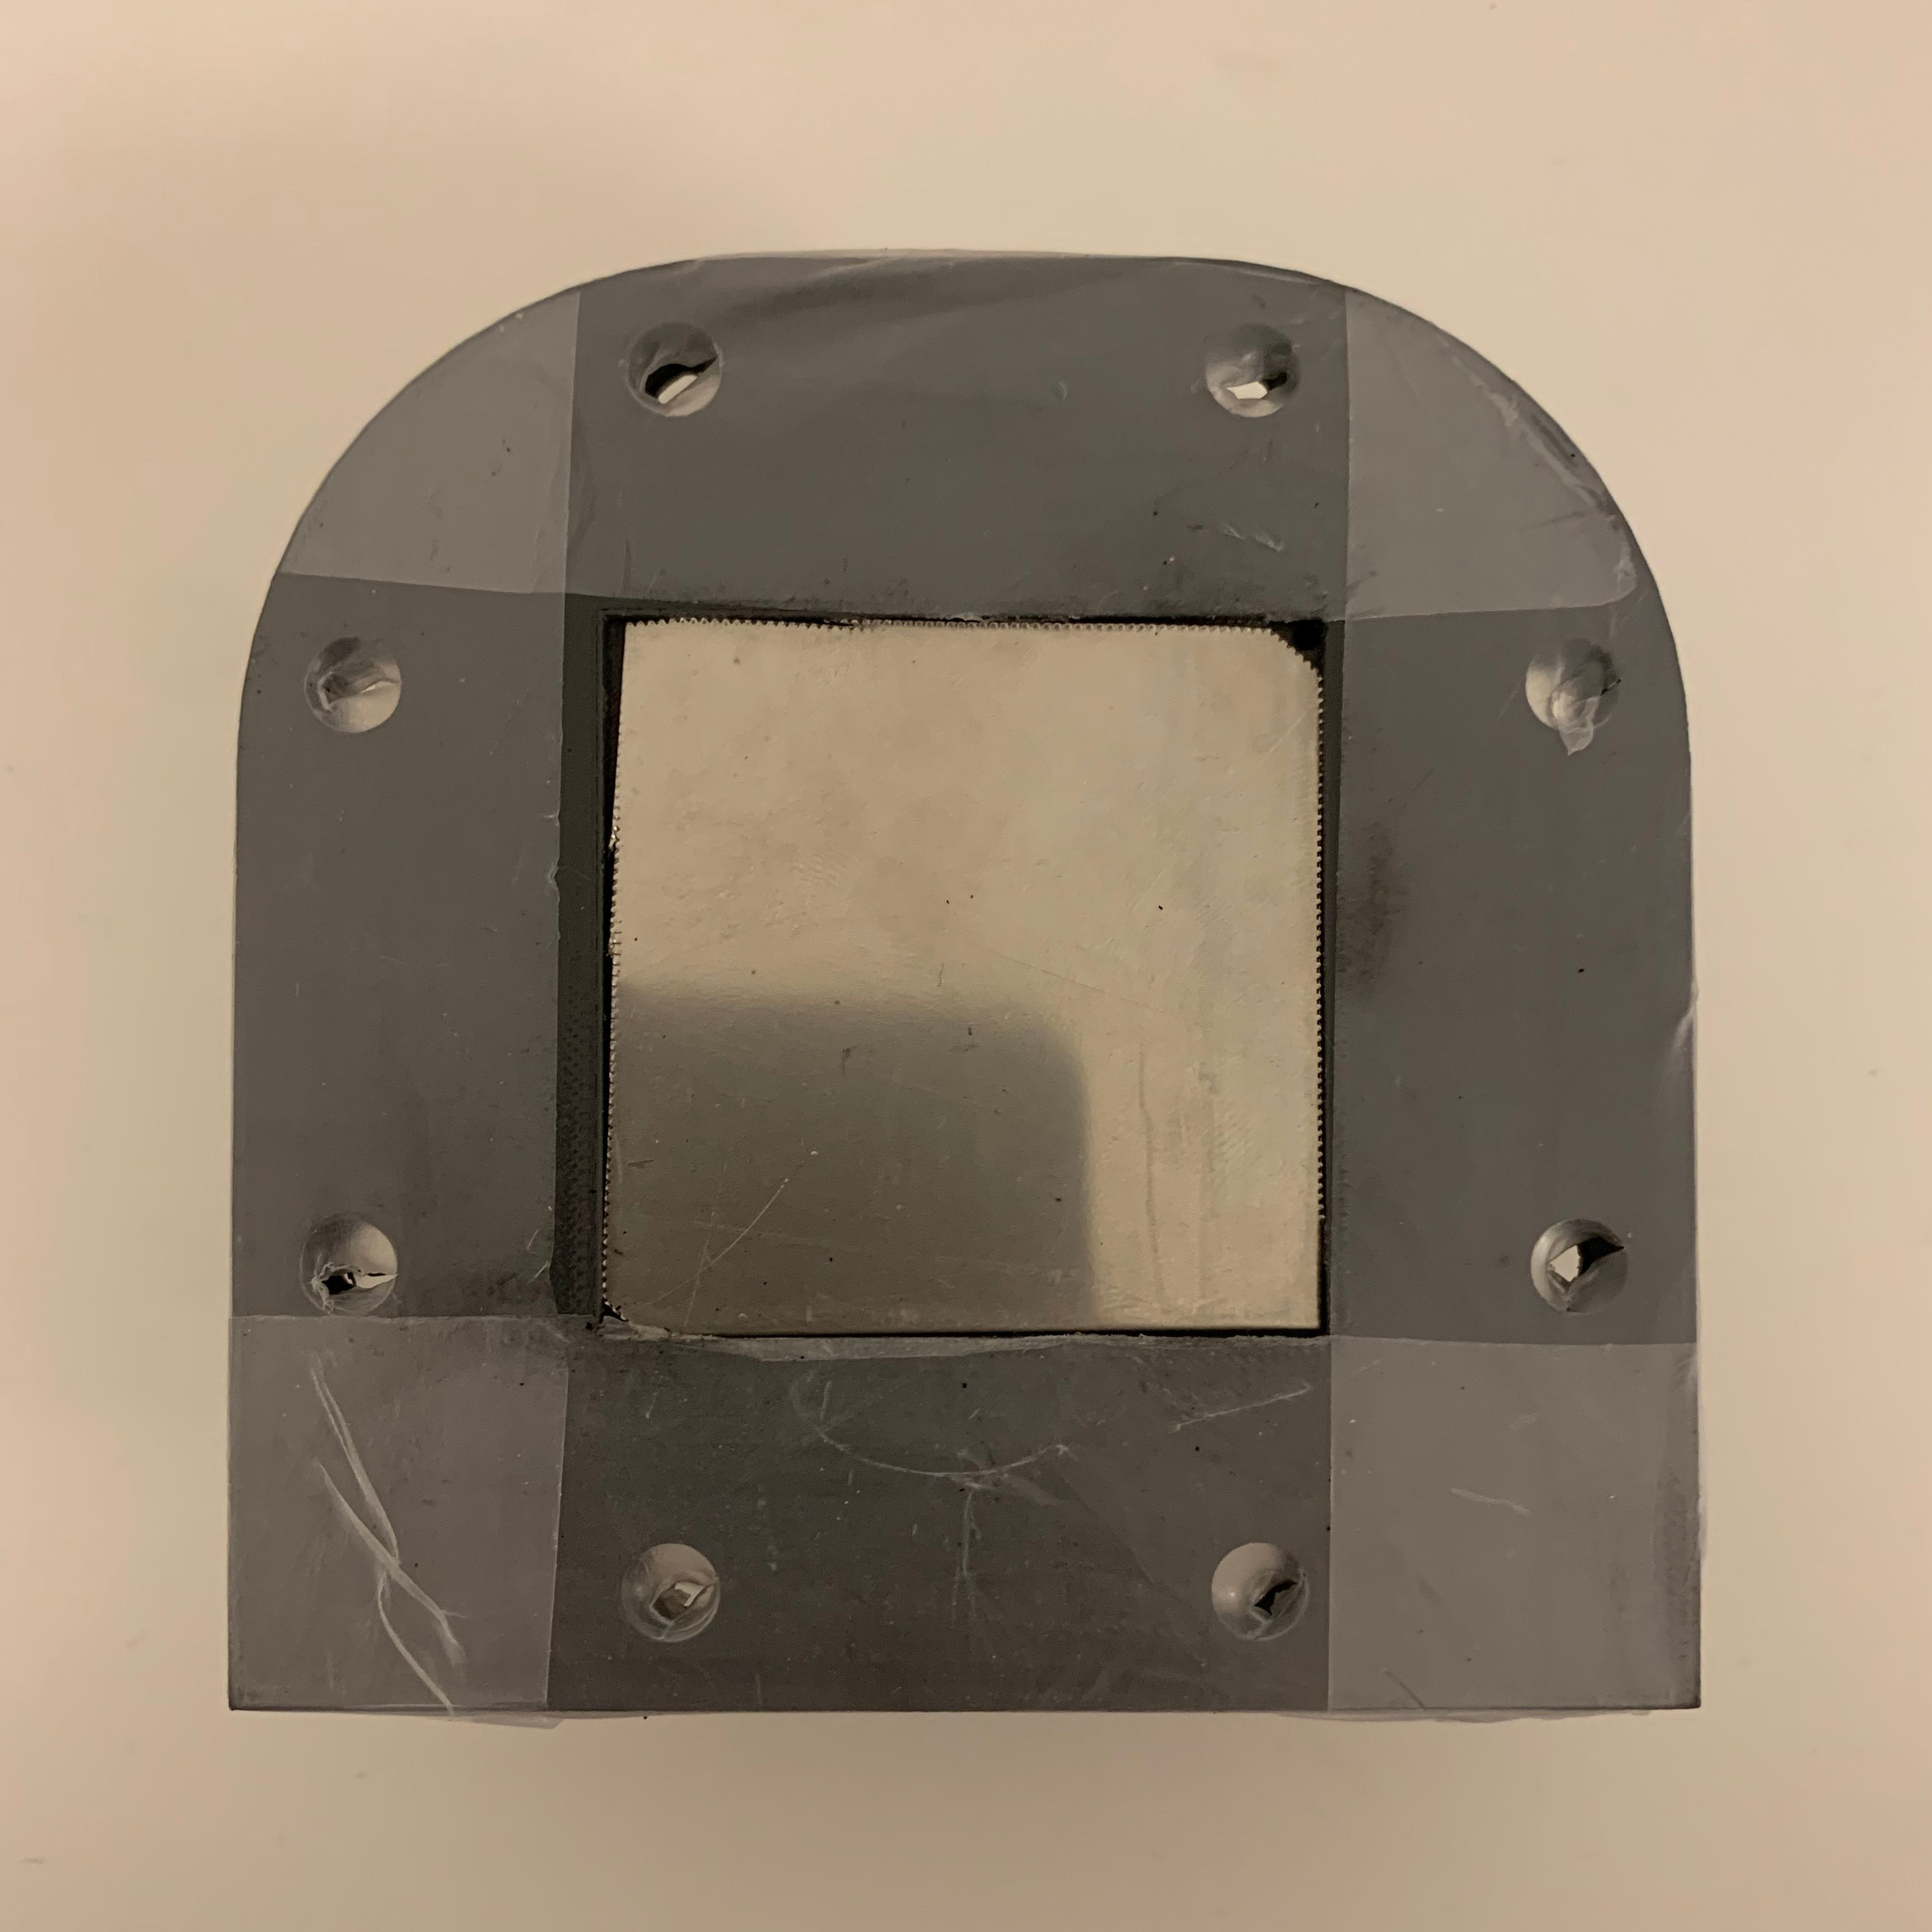
\includegraphics[width=\textwidth]{DIV./Bilder/Assembly/Ass1.jpg}
        \caption{Metalplate and Parafilm gas seal}
        \label{fig:GasSealMetal}
    \end{subfigure}
    ~ %add desired spacing between images, e. g. ~, \quad, \qquad, \hfill etc. 
      %(or a blank line to force the subfigure onto a new line)
    \begin{subfigure}[b]{0.3\textwidth}
        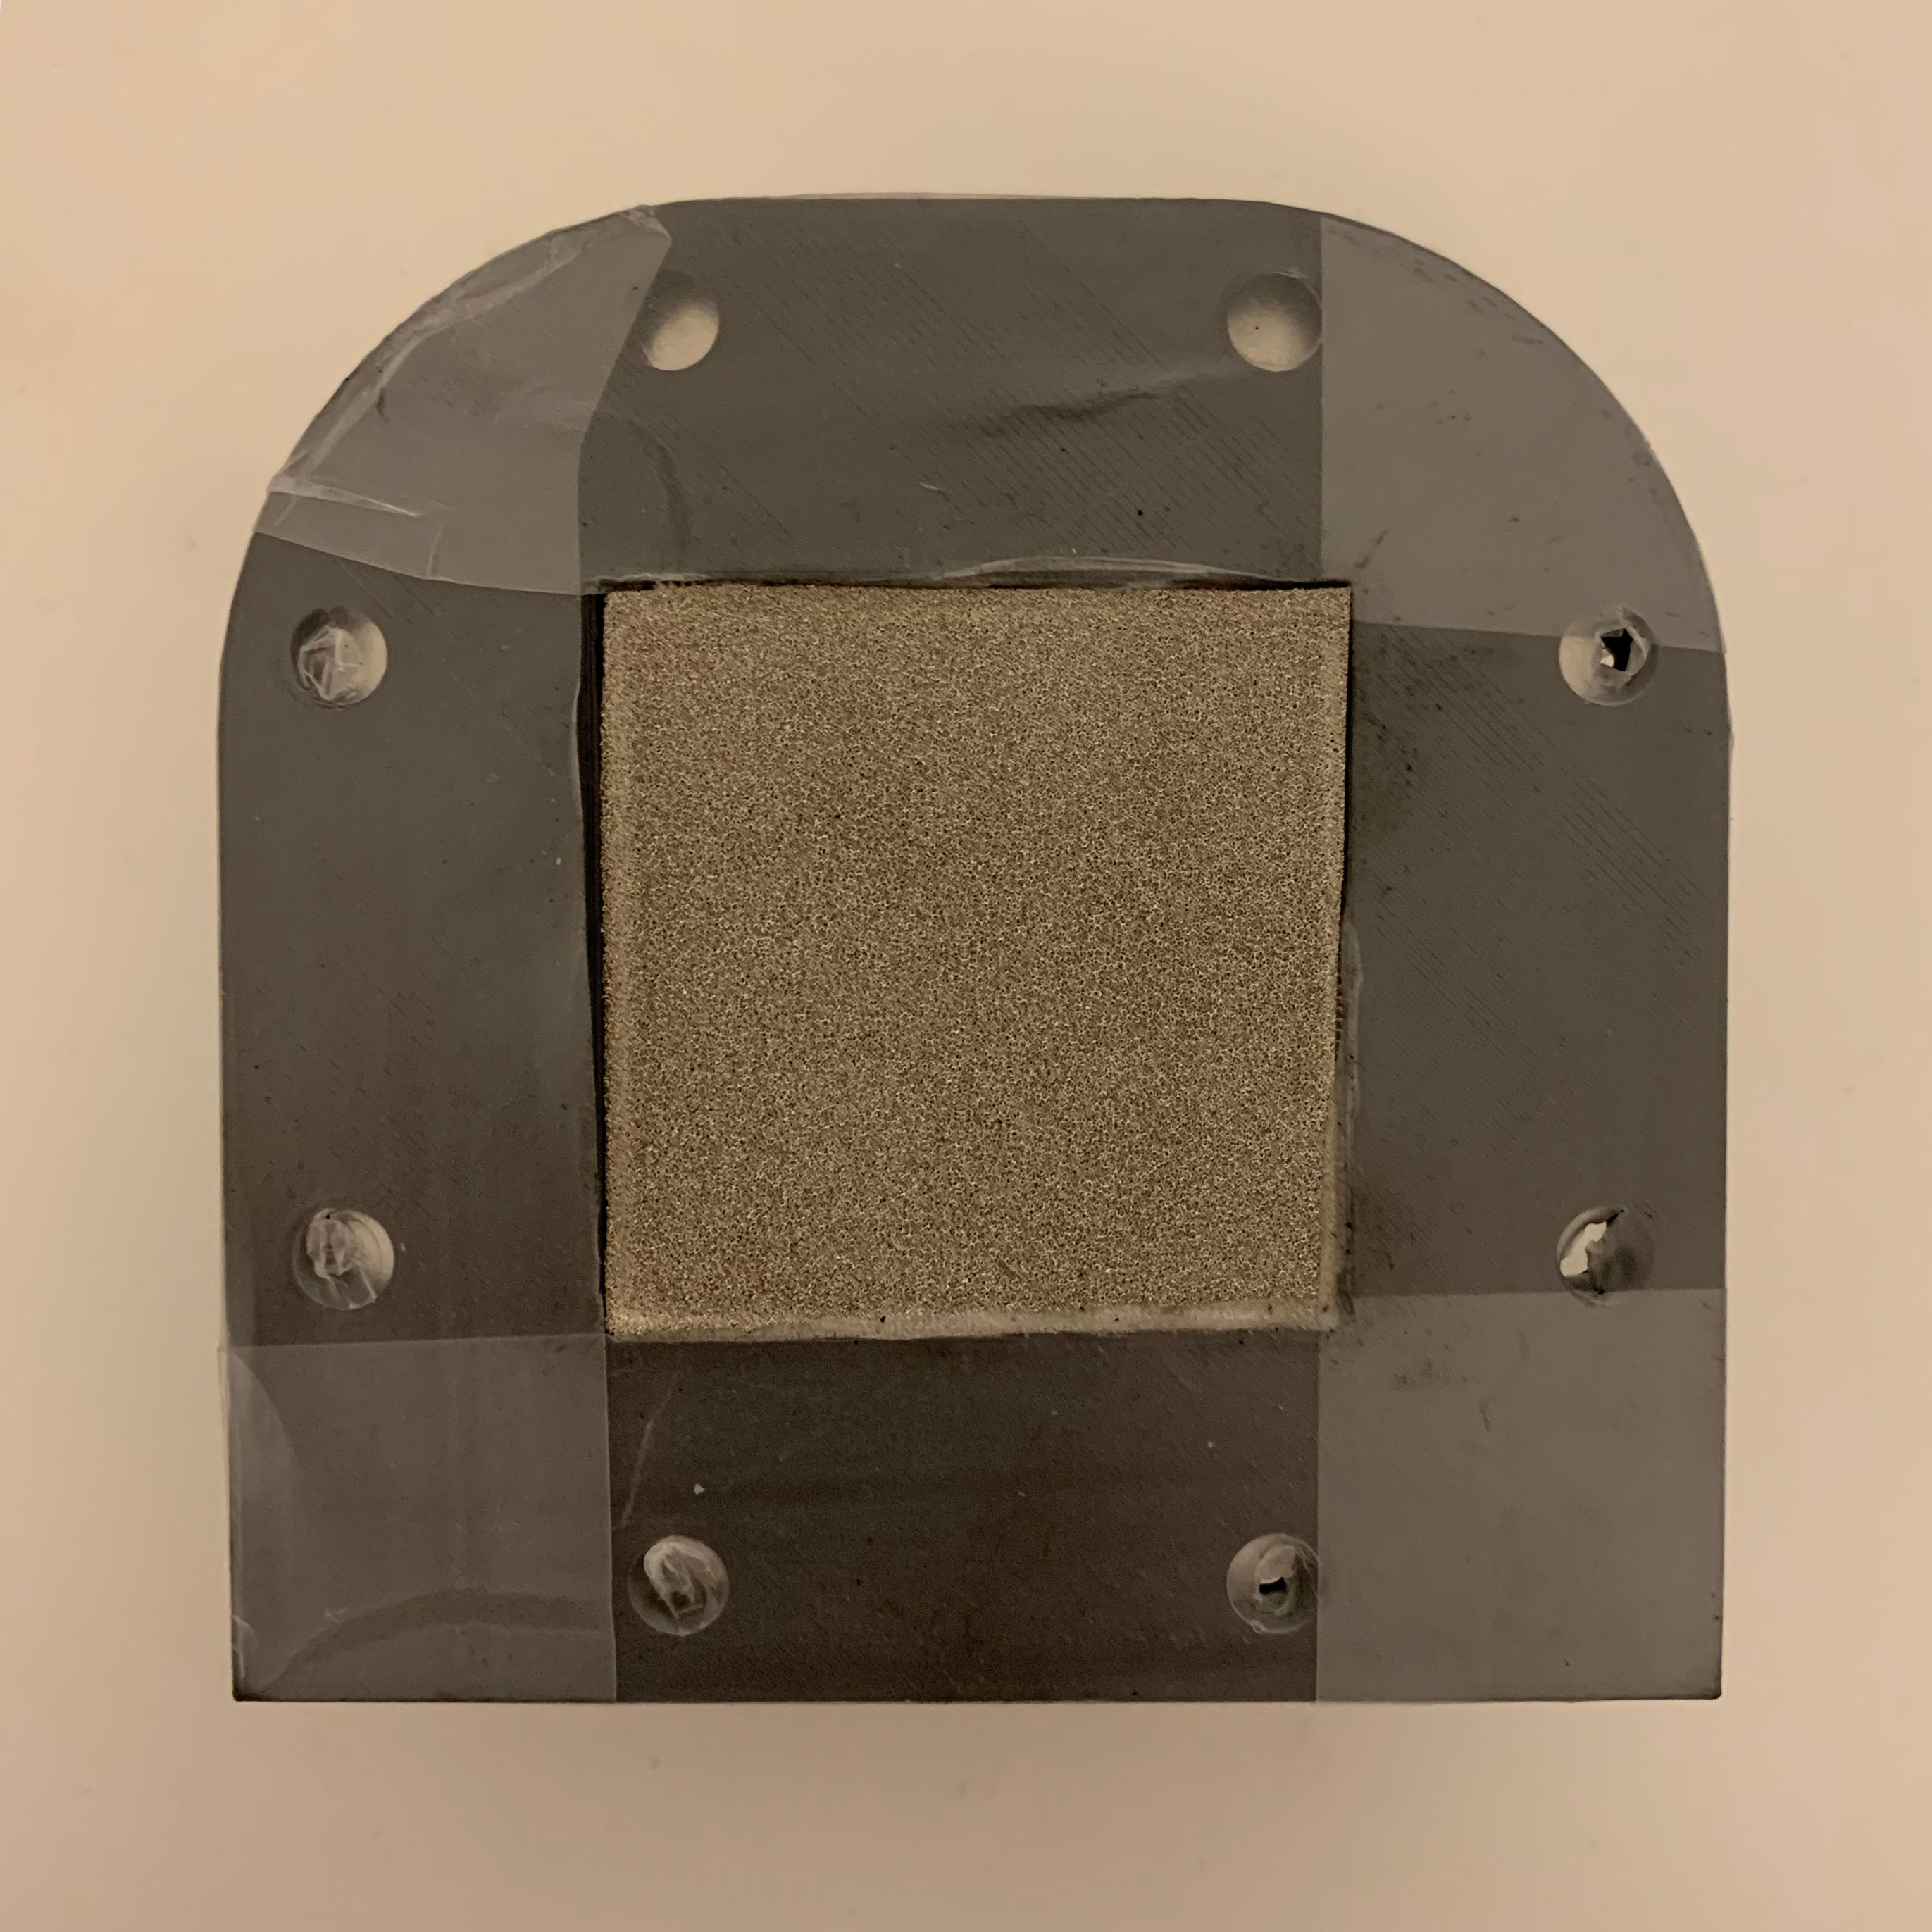
\includegraphics[width=\textwidth]{DIV./Bilder/Assembly/Ass2.jpg}
        \caption{Nickel foam gas diffusion layer}
        \label{fig:NickelFoam}
    \end{subfigure}
    ~ %add desired spacing between images, e. g. ~, \quad, \qquad, \hfill etc. 
    %(or a blank line to force the subfigure onto a new line)
    \begin{subfigure}[b]{0.3\textwidth}
        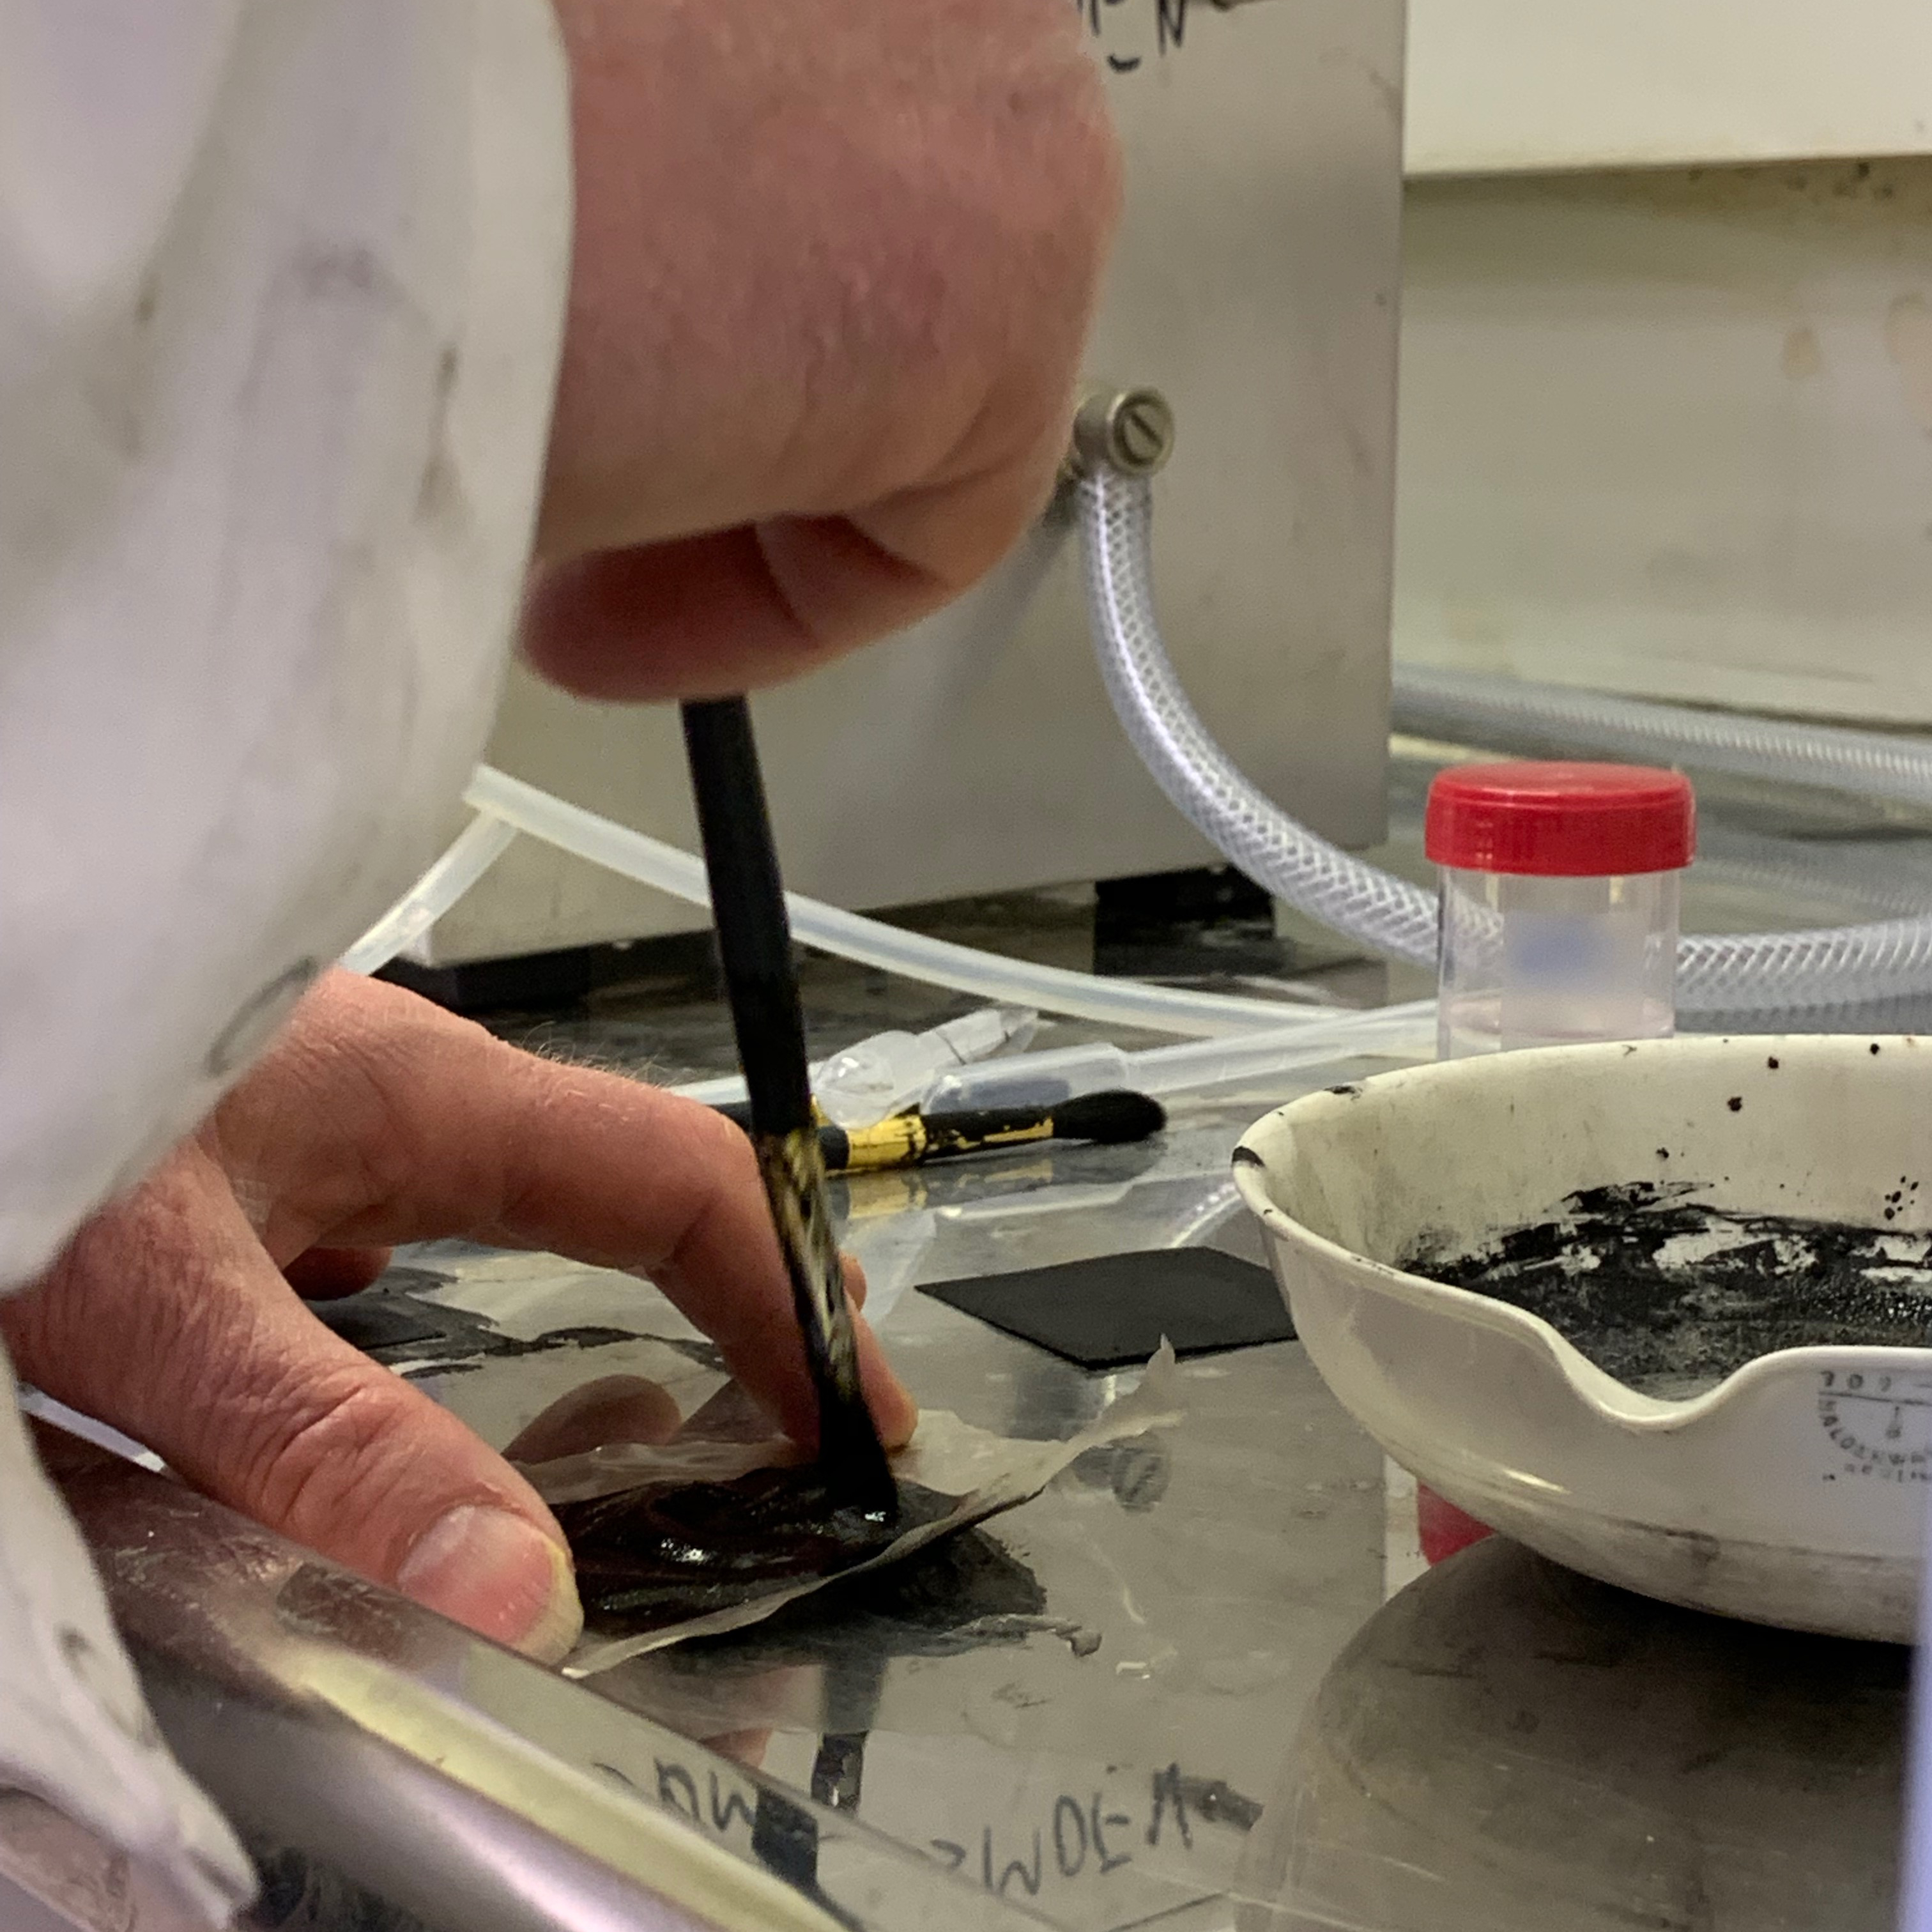
\includegraphics[width=\textwidth]{DIV./Bilder/Assembly/Ass3.jpg}
        \caption{Catalyst painted on membrane}
        \label{fig:CatalystPaint}
    \end{subfigure}
    \caption{Assembly of the metalplate, nickel foam and Parafilm}\label{fig:Assembly1}
\end{figure}

On top of the metal plate we placed the nickel foam. The nickel foam is used as a gas diffusion layer. The gas diffusion layer is used to spread the gas molecules better so that more reactions can happen at the same time. Due to the height of the nickel foam, and the little space in the PEMFC, the nickel foam was softly hammered flatter to make it fit. After flattening the nickel foam, it was cut to fit inside the fuel cell. This can be seen on figure \ref{fig:NickelFoam}.

The catalyst was then painted on the Nafion membrane and on the carbon electrodes. The carbon-platinum blend was mixed with isopropyl alcohol (IPA) to make the catalyst a thin liquid. This was done to make the catalyst easy to apply with a paintbrush, as seen on figure \ref{fig:CatalystPaint}. When left to dry the alcohol evaporated and left the catalyst on the membrane and on the carbon paper electrolytes. To quickly dry the membrane and the electrodes a heating plat was used. When the catalyst and the electrodes was dry they were added to the fuel cell. First an electrode was added then the membrane and on top of that the next electrode. This can be seen in figure \ref{fig:ElectrodeMembraneAssembly}


\begin{figure}[ht]
    \centering
    \begin{subfigure}[b]{0.3\textwidth}
        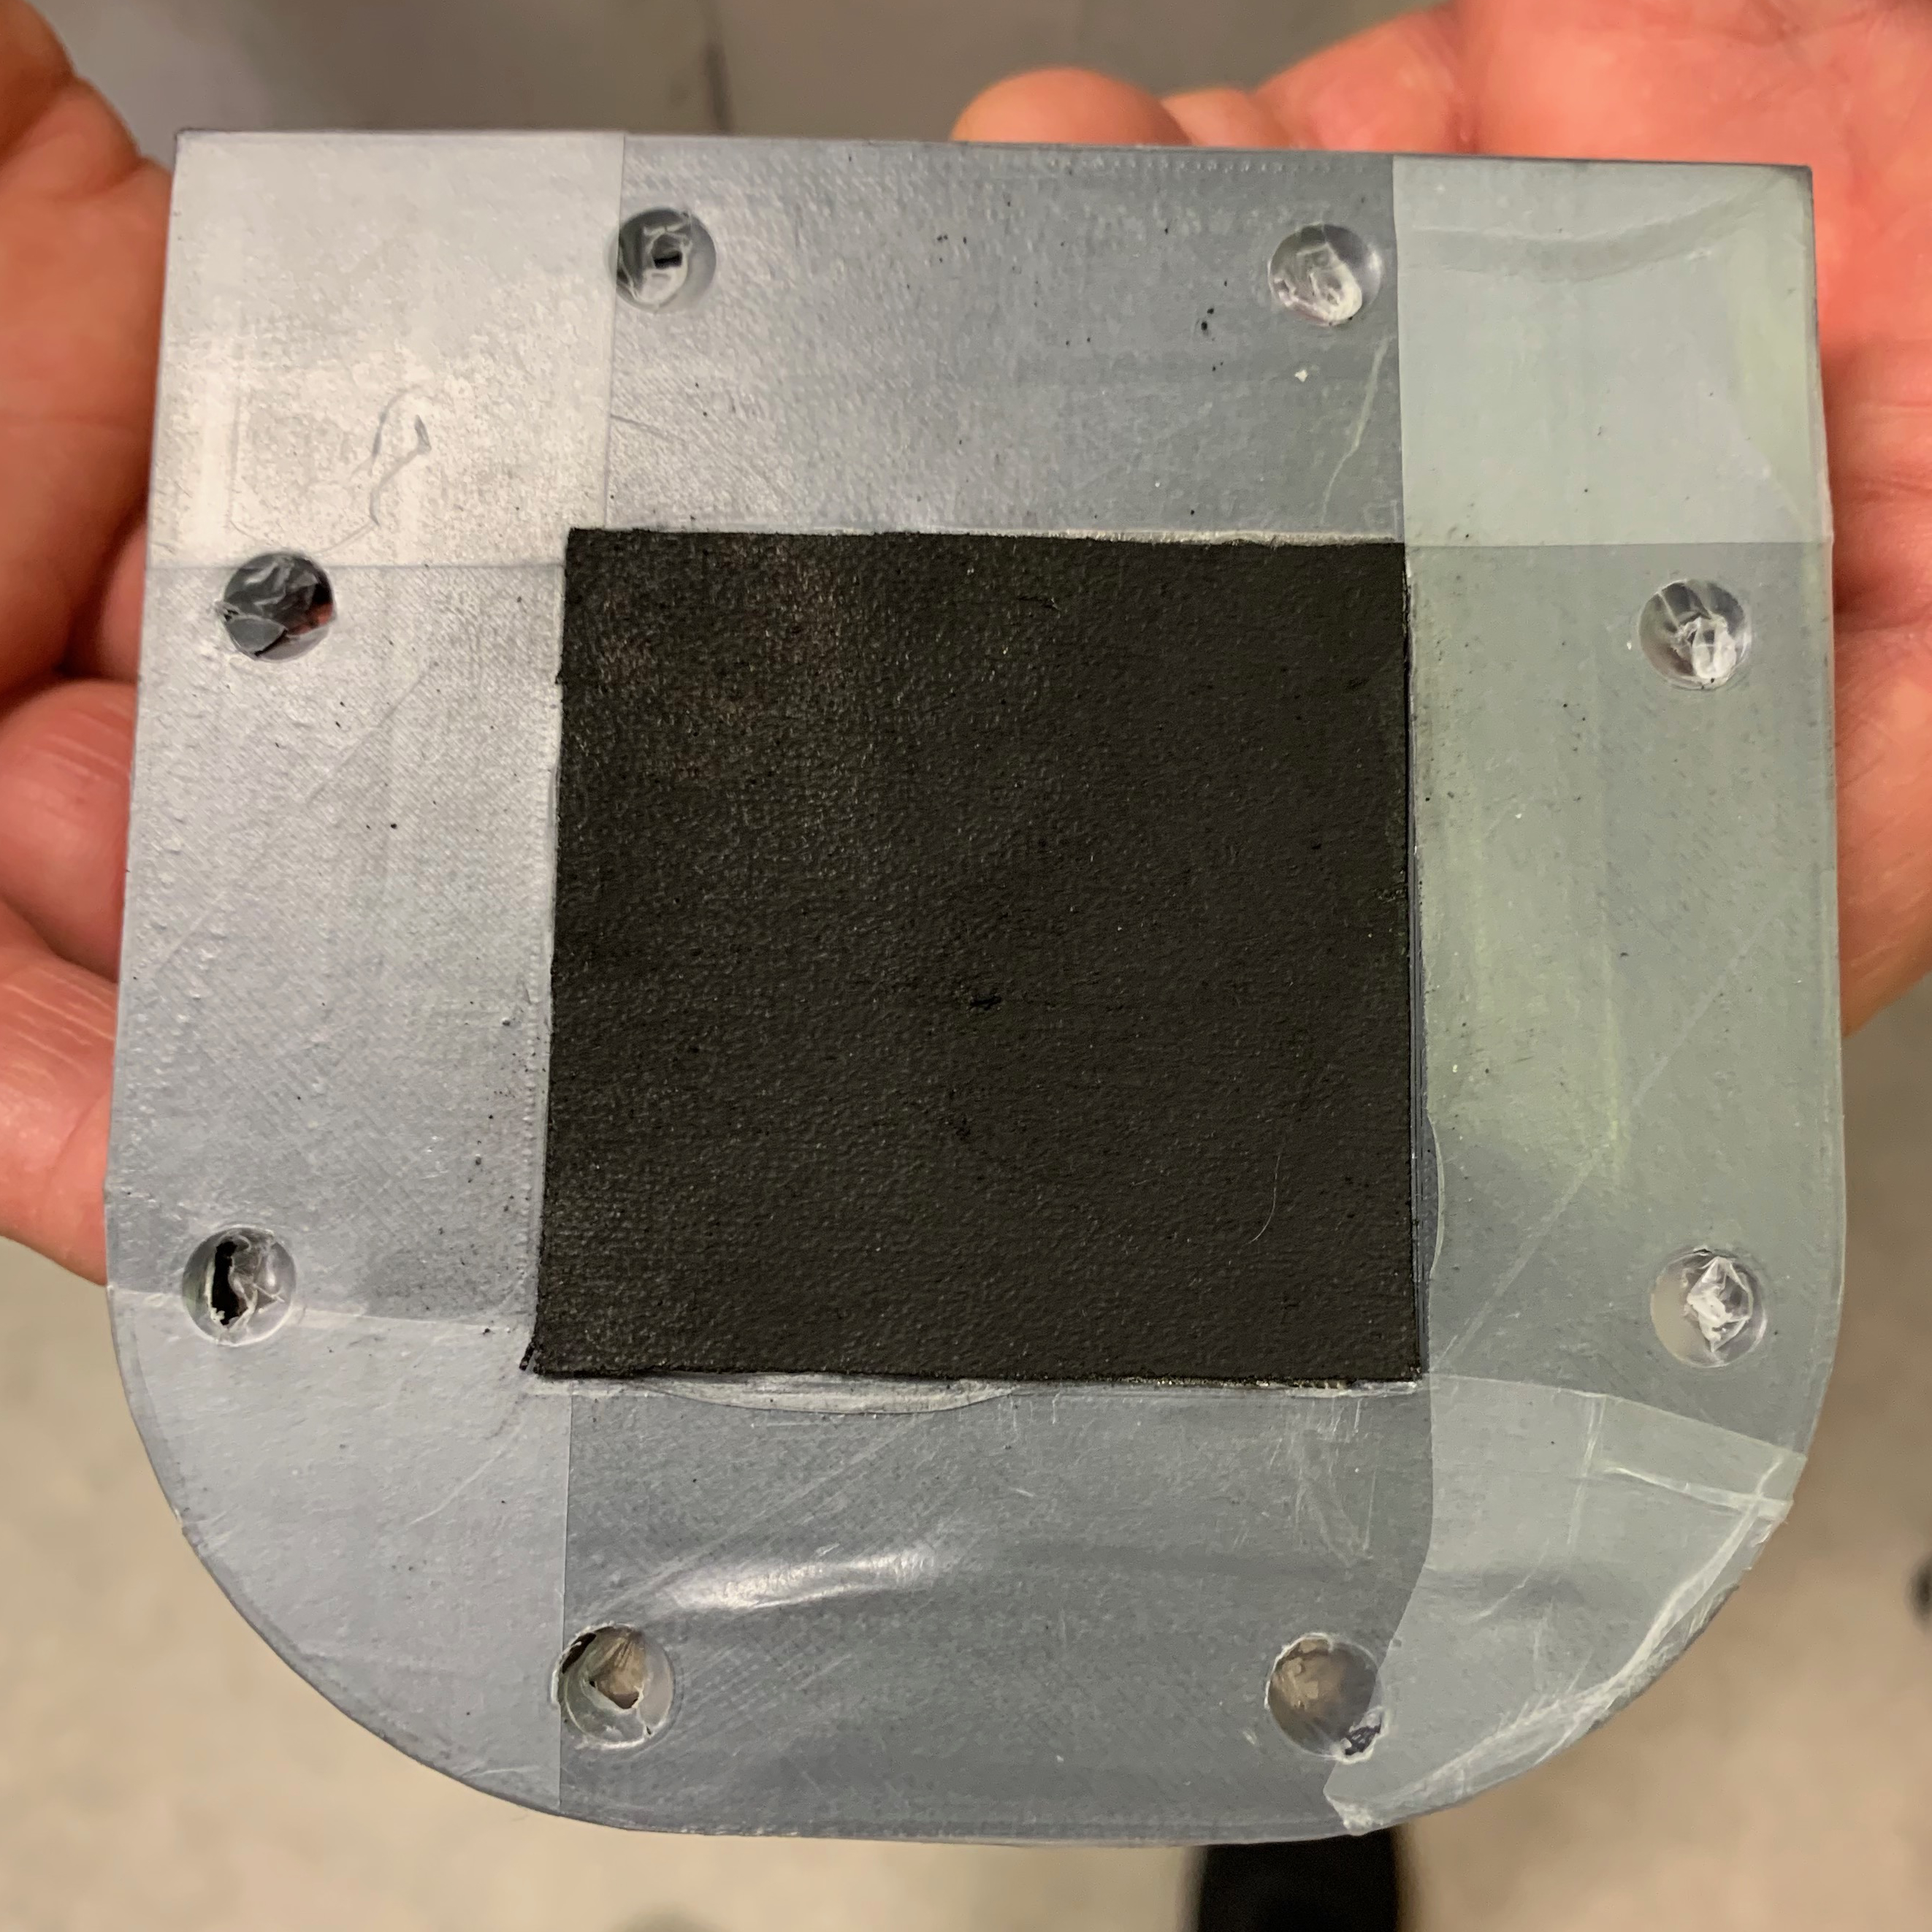
\includegraphics[width=\textwidth]{DIV./Bilder/Assembly/Ass4.jpg}
        \caption{The first electrolyte placed on top of the nickel foam}
        \label{fig:1Electrode}
    \end{subfigure}
    ~ %add desired spacing between images, e. g. ~, \quad, \qquad, \hfill etc. 
      %(or a blank line to force the subfigure onto a new line)
    \begin{subfigure}[b]{0.3\textwidth}
        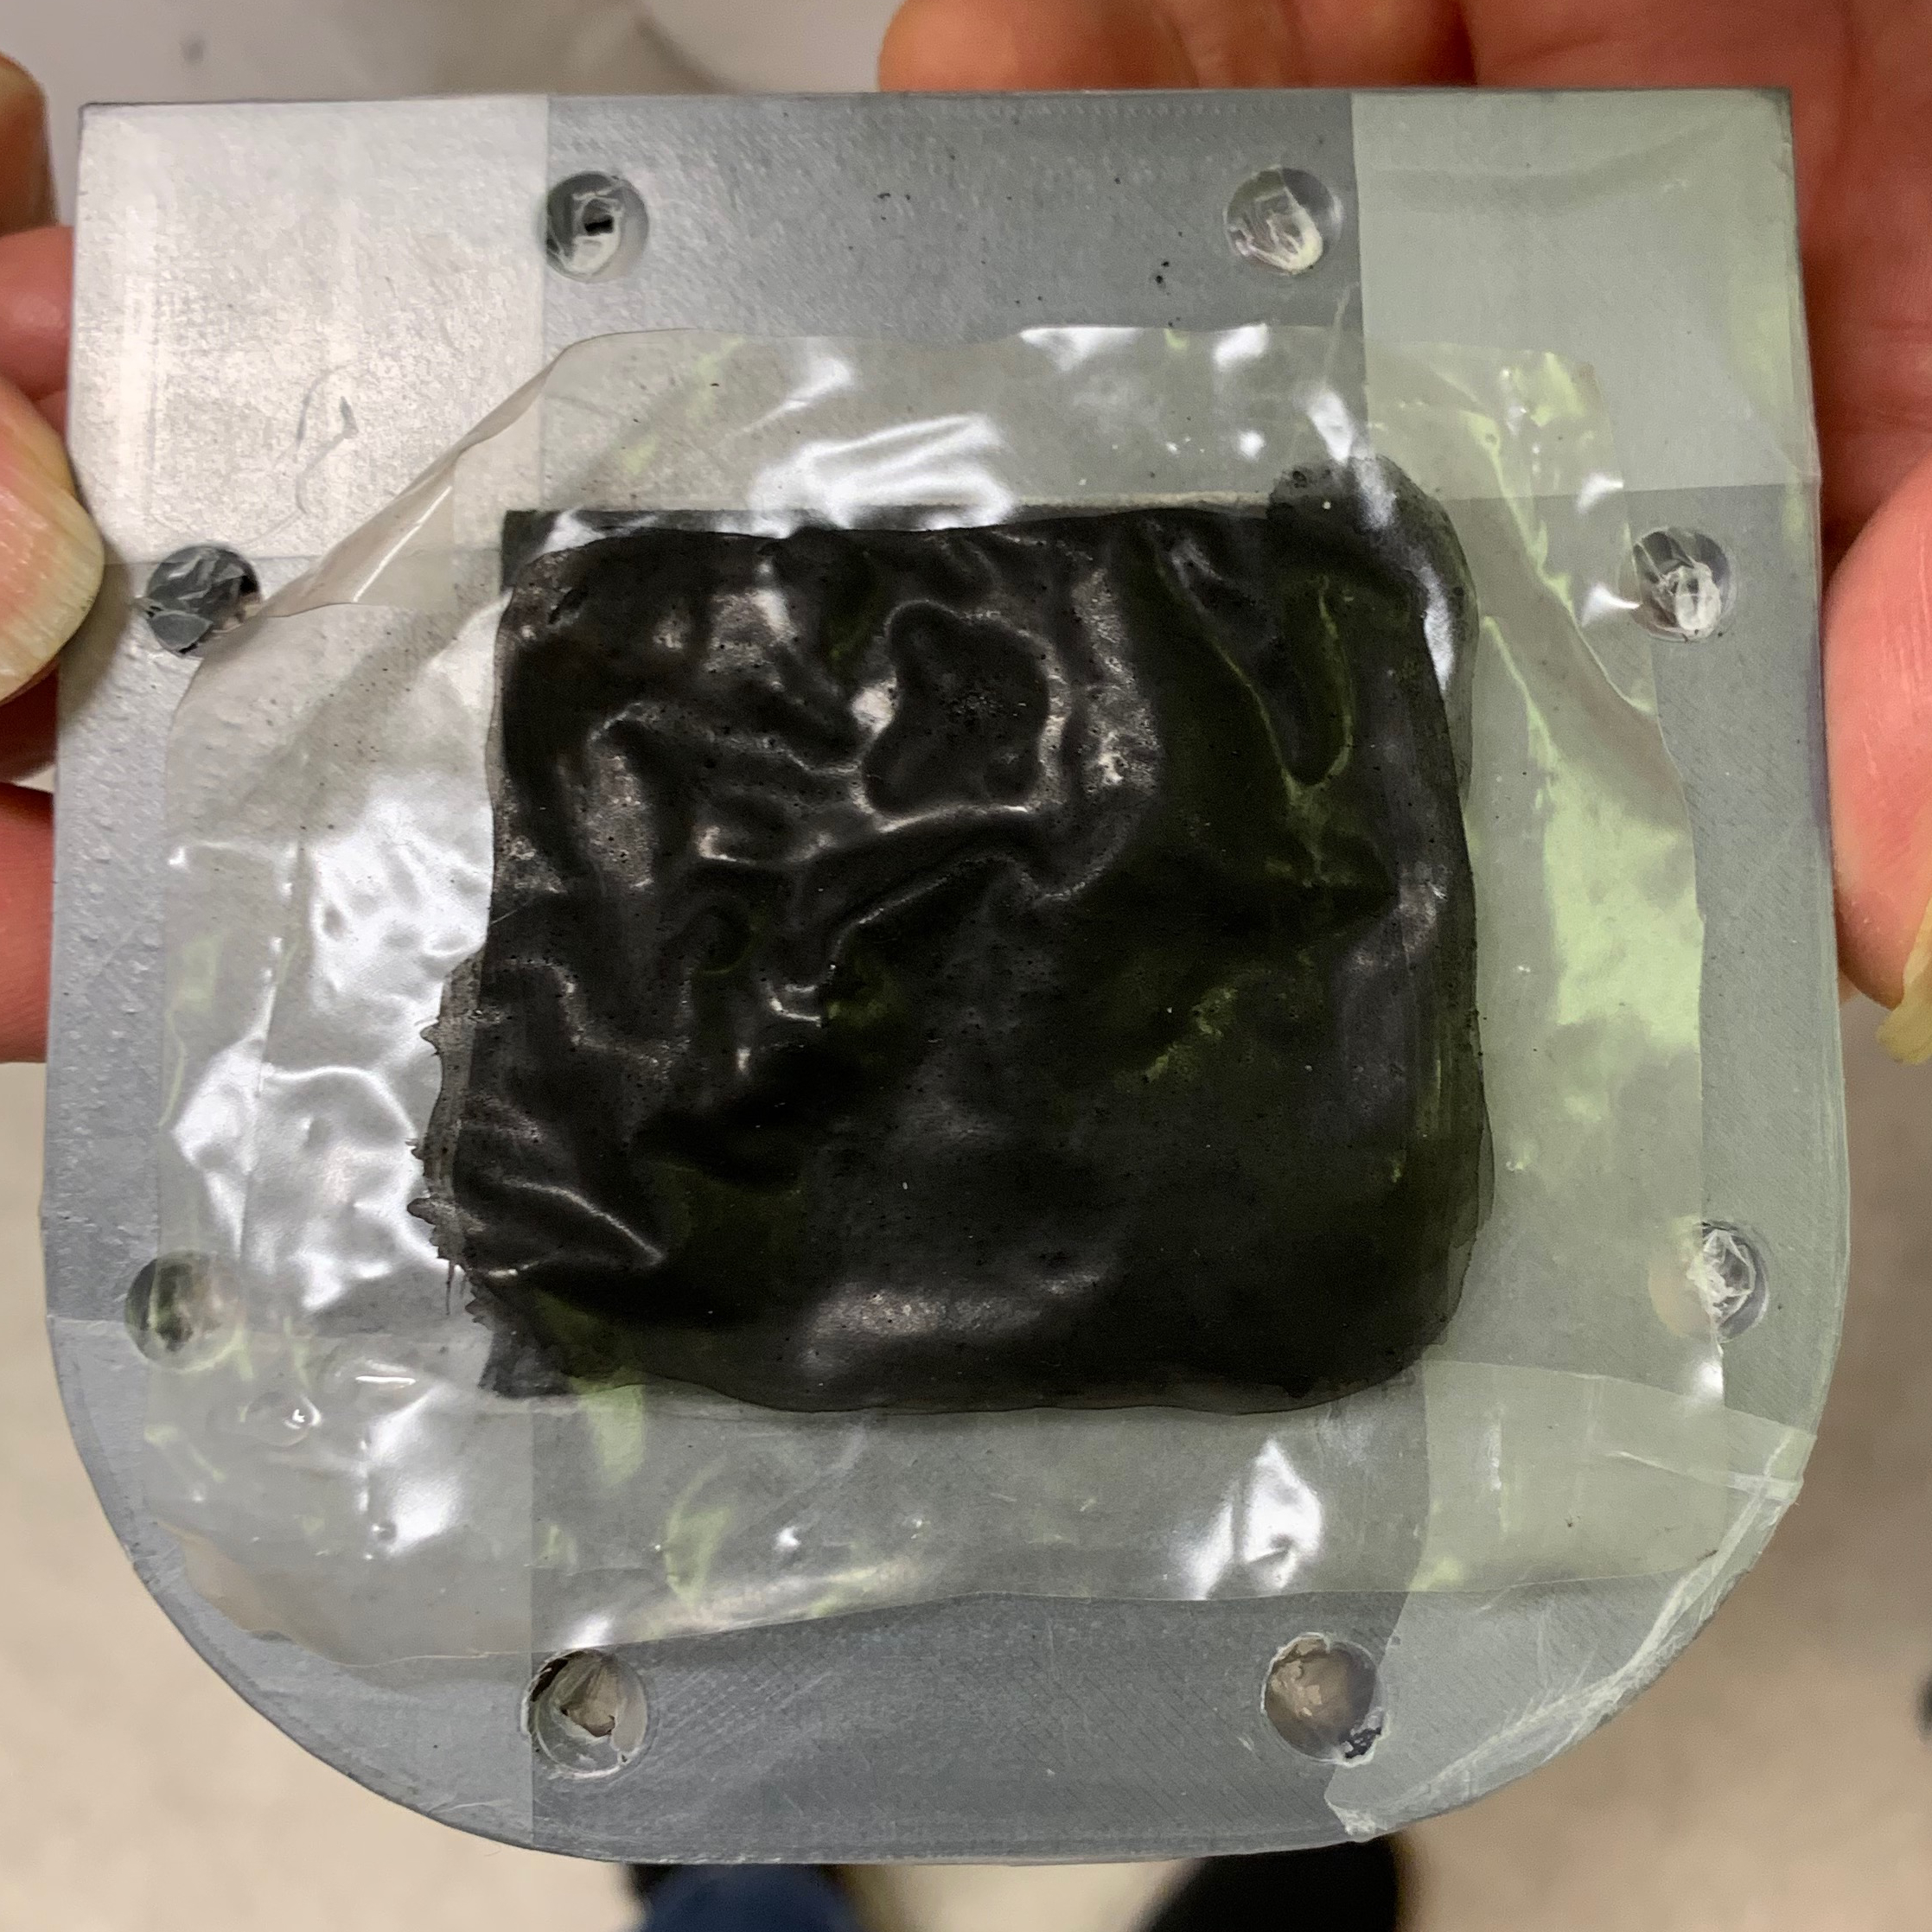
\includegraphics[width=\textwidth]{DIV./Bilder/Assembly/Ass5.jpg}
        \caption{The membrane inside the fuel cell}
        \label{fig:Membrane}
    \end{subfigure}
    ~ %add desired spacing between images, e. g. ~, \quad, \qquad, \hfill etc. 
    %(or a blank line to force the subfigure onto a new line)
    \begin{subfigure}[b]{0.3\textwidth}
        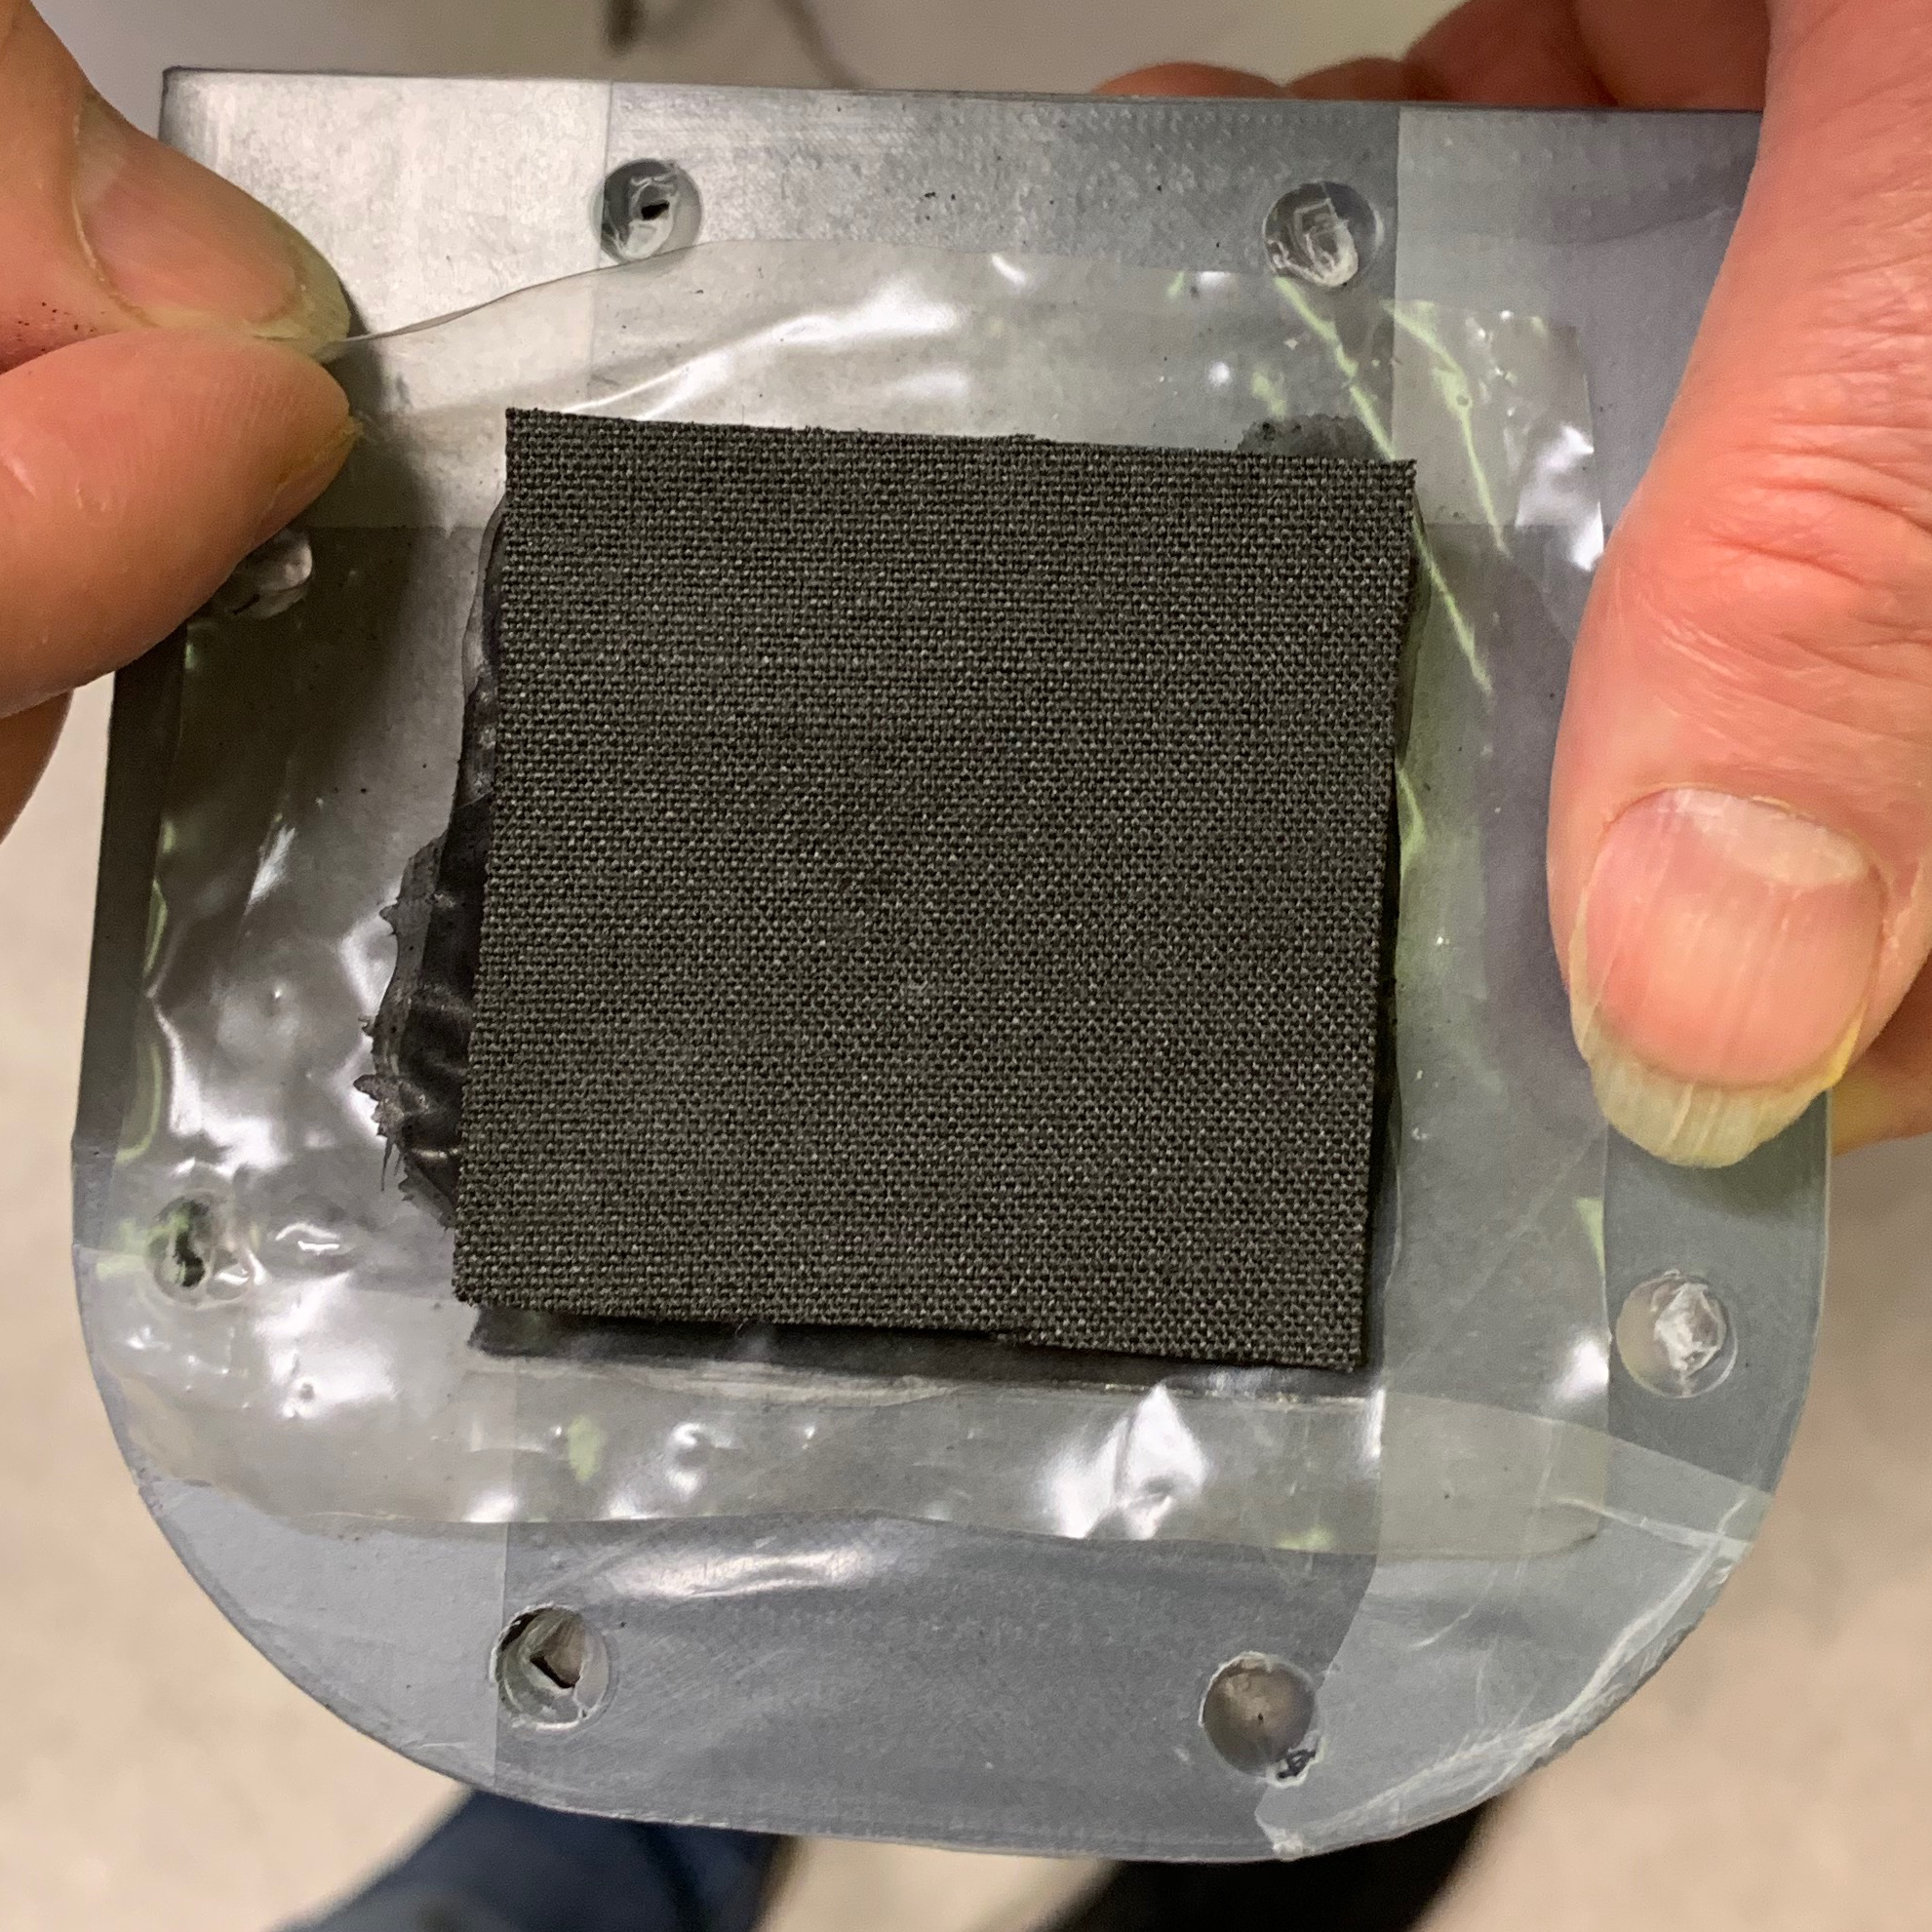
\includegraphics[width=\textwidth]{DIV./Bilder/Assembly/Ass6.jpg}
        \caption{The second electrode placed inside the fuel cell}
        \label{fig:2Electrode}
    \end{subfigure}
    \caption{Assembly of the electrodes and membrane}\label{fig:ElectrodeMembraneAssembly}
\end{figure}

The other side of the housing was then added and fastened together by eight M8 bolts and nuts. The bolts and nuts where tightened to make sure no gas could leak outside of the fuel cell. A bigger bolt, M12, was screwed in the middle of the fuel cell. We added Teflon tape on the end of the bolt to make sure it was an air tight fit. The M12 bolt was screwed in until it touched the metal plates inside the fuel cell. We could then use the M12 bolt to collect the voltage generated by the fuel cell. At the end a piece of tape was put on one side of the fuel cell to mark what side hydrogen should enter. The finished fuel cell can be seen on figure \ref{fig:FinishedFuelCell}.

\begin{figure}[ht]
    \centering
    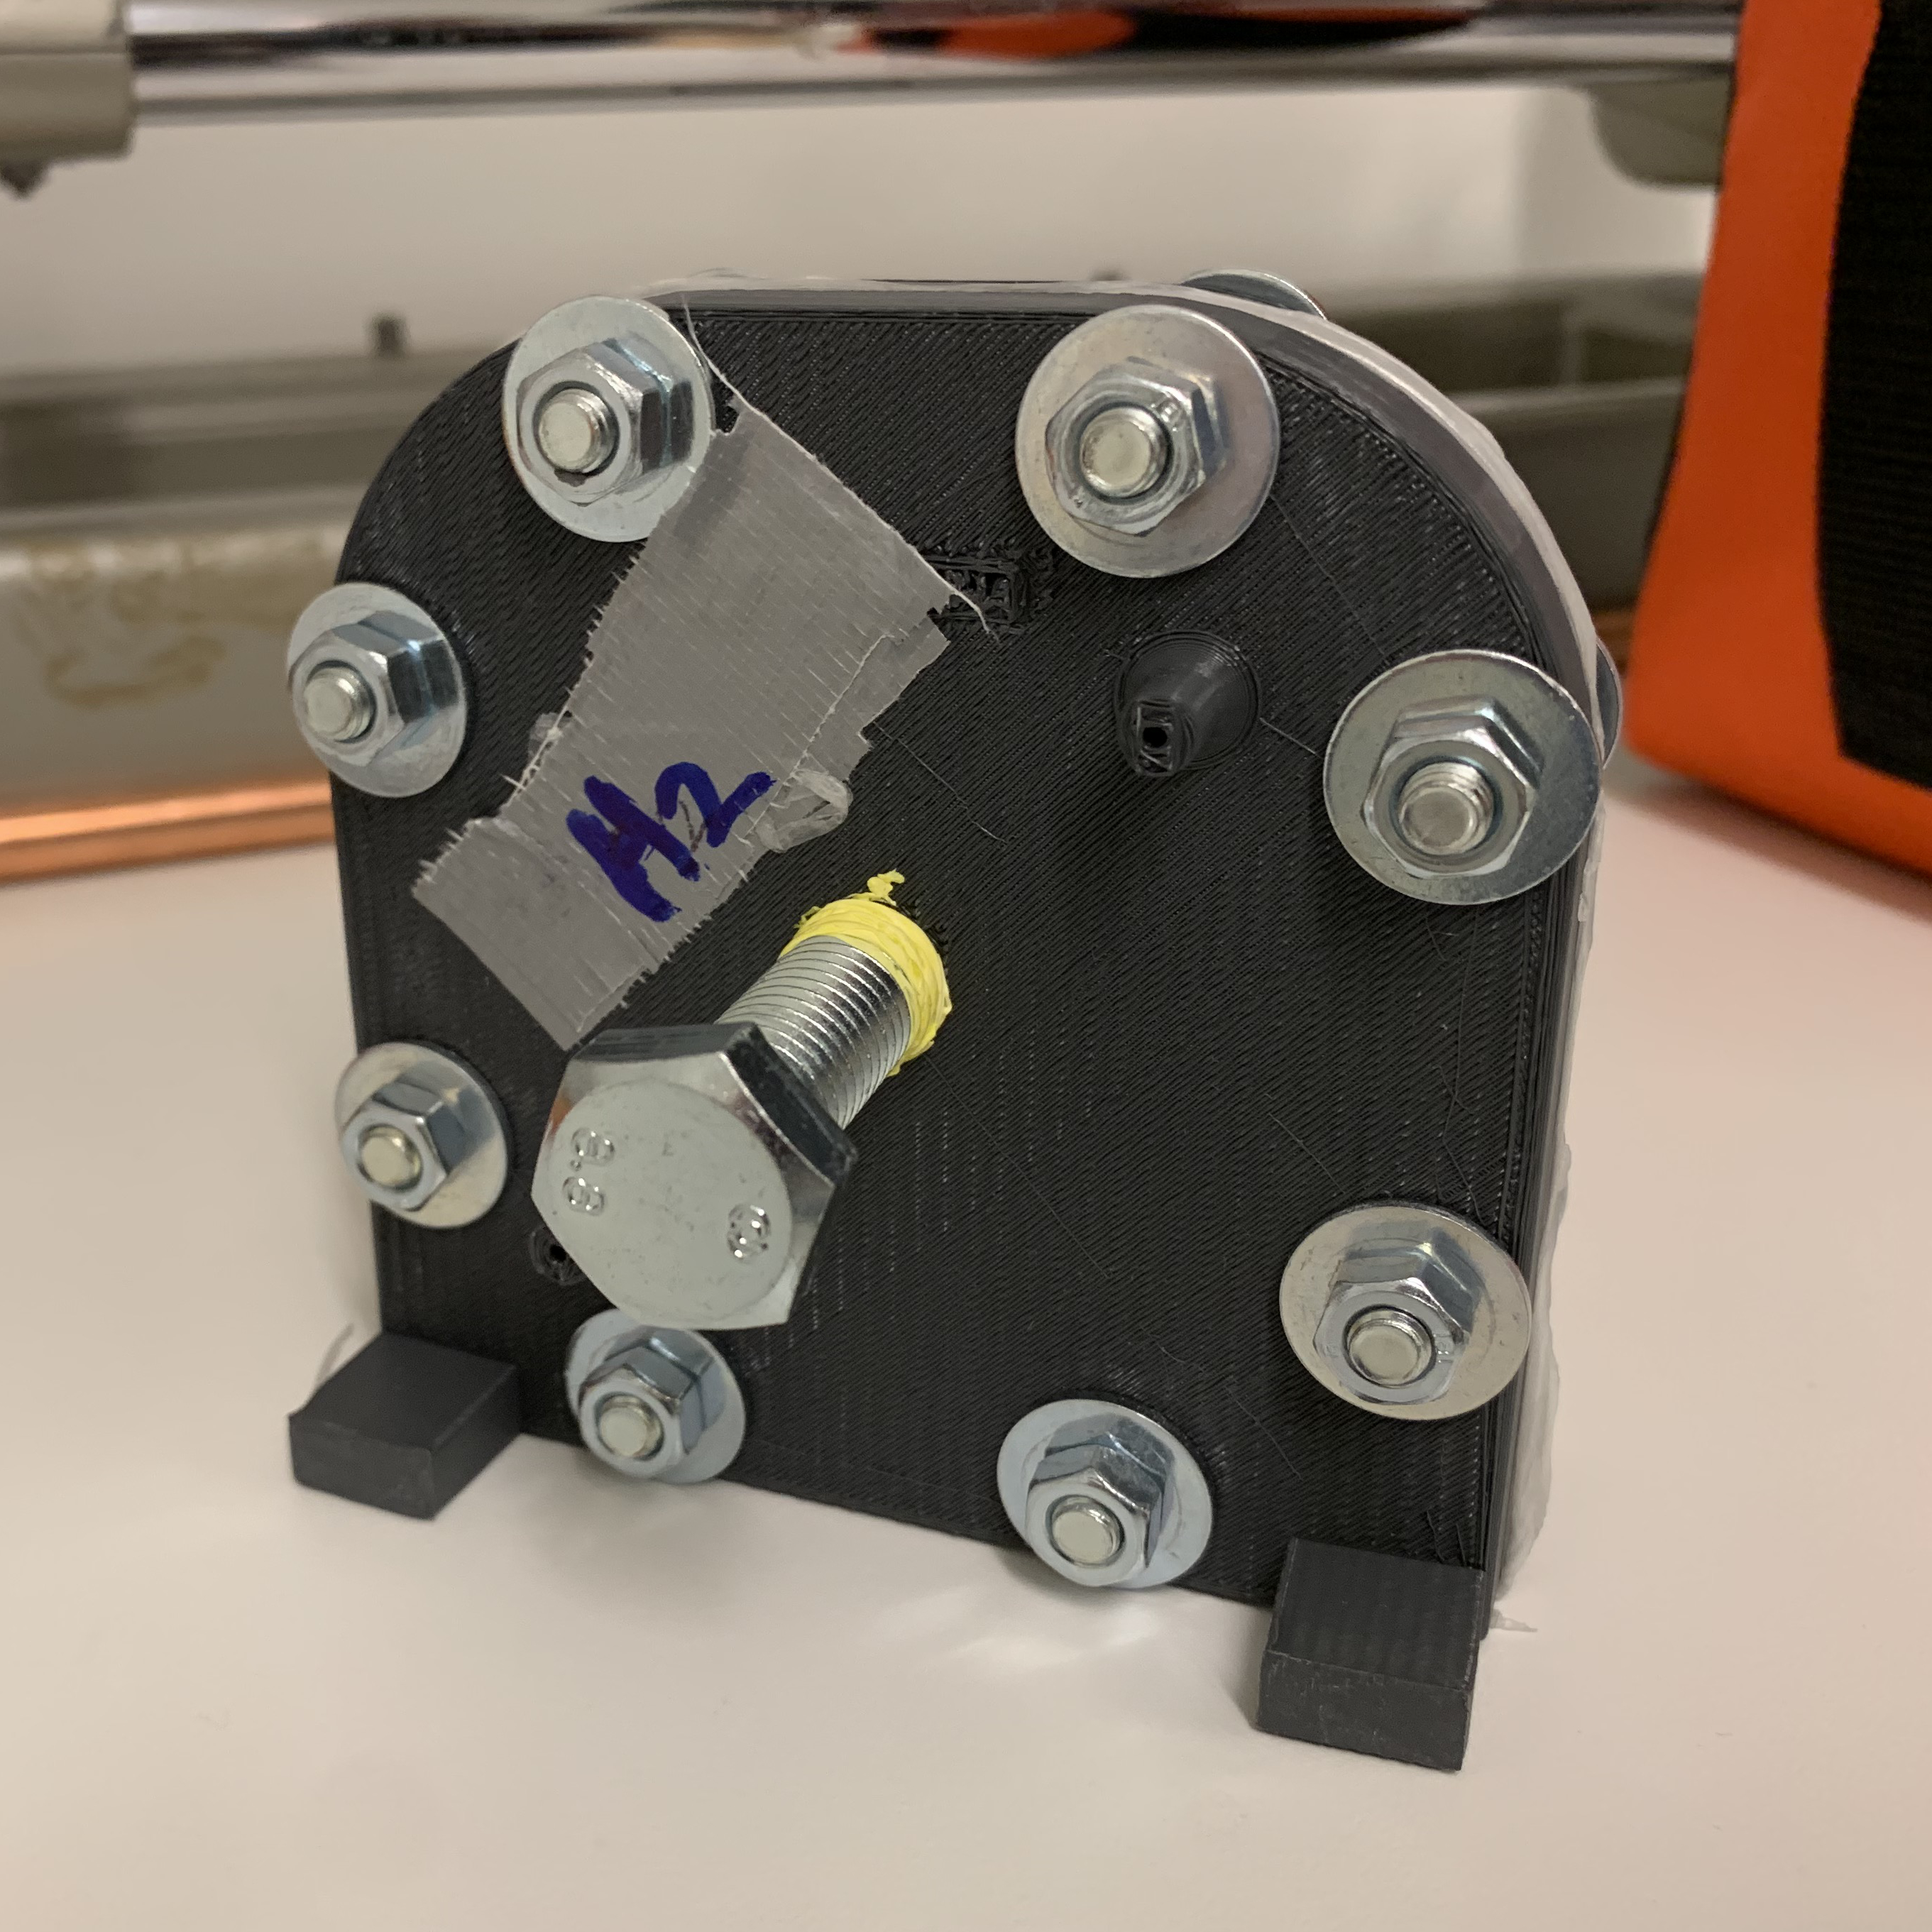
\includegraphics[width=0.4\textwidth]{DIV./Bilder/Assembly/Fuelcell.jpg}
    \caption{The fully assembled PEM fuel cell}
    \label{fig:FinishedFuelCell}
\end{figure}

\section{Testing}

The fuel cell was supplied with hydrogen from an outlet that was connected, through pipes, to hydrogen storage tanks. Oxygen was supplied through air that was pumped by an electric air-pump to create a continuous flow through the fuel cell. Both gasses were supply via tubes that was connected to the bottom tap on their respective sides of the fuel cell. Exit tubes were connected to the top taps while the other ends of the was placed in water, this way we could visually verify that there was a flow of gas. We connected the fuel cell to a load bank to easily be able to change between loads during our tests. Two voltmeters were used in the setup, one was placed to measure voltage over the fuel cell itself while the other was placed to measure voltage over the load.

We started the tests by measuring open circuit voltage, and proceeded by connecting a load-bank and measured the voltage over the first load step at 10.000 ohms. The load was decreased step by step while measuring voltage at each step.
 
We tested the fuel cell in four different setups. The first and second test was done using nickel foam as gas distribution layer inside of the fuel cell. The first test the fuel cell was dry, for the second test we filled the cell with water to soak the electrolyte. For the third and fourth tests, we took out the nickel distribution layer and repeated the testing process as was done in previous tests. This was done to test how well the fuel cell performed with the nickel foam distribution layer versus with only the carbon paper as a diffusion layer.

To make sure that the electrolyte was completely dry between the wet tests and the dry tests we placed it on a hotplate, on low heat, to make the water evaporate.

\begin{figure}[ht]
    \centering
    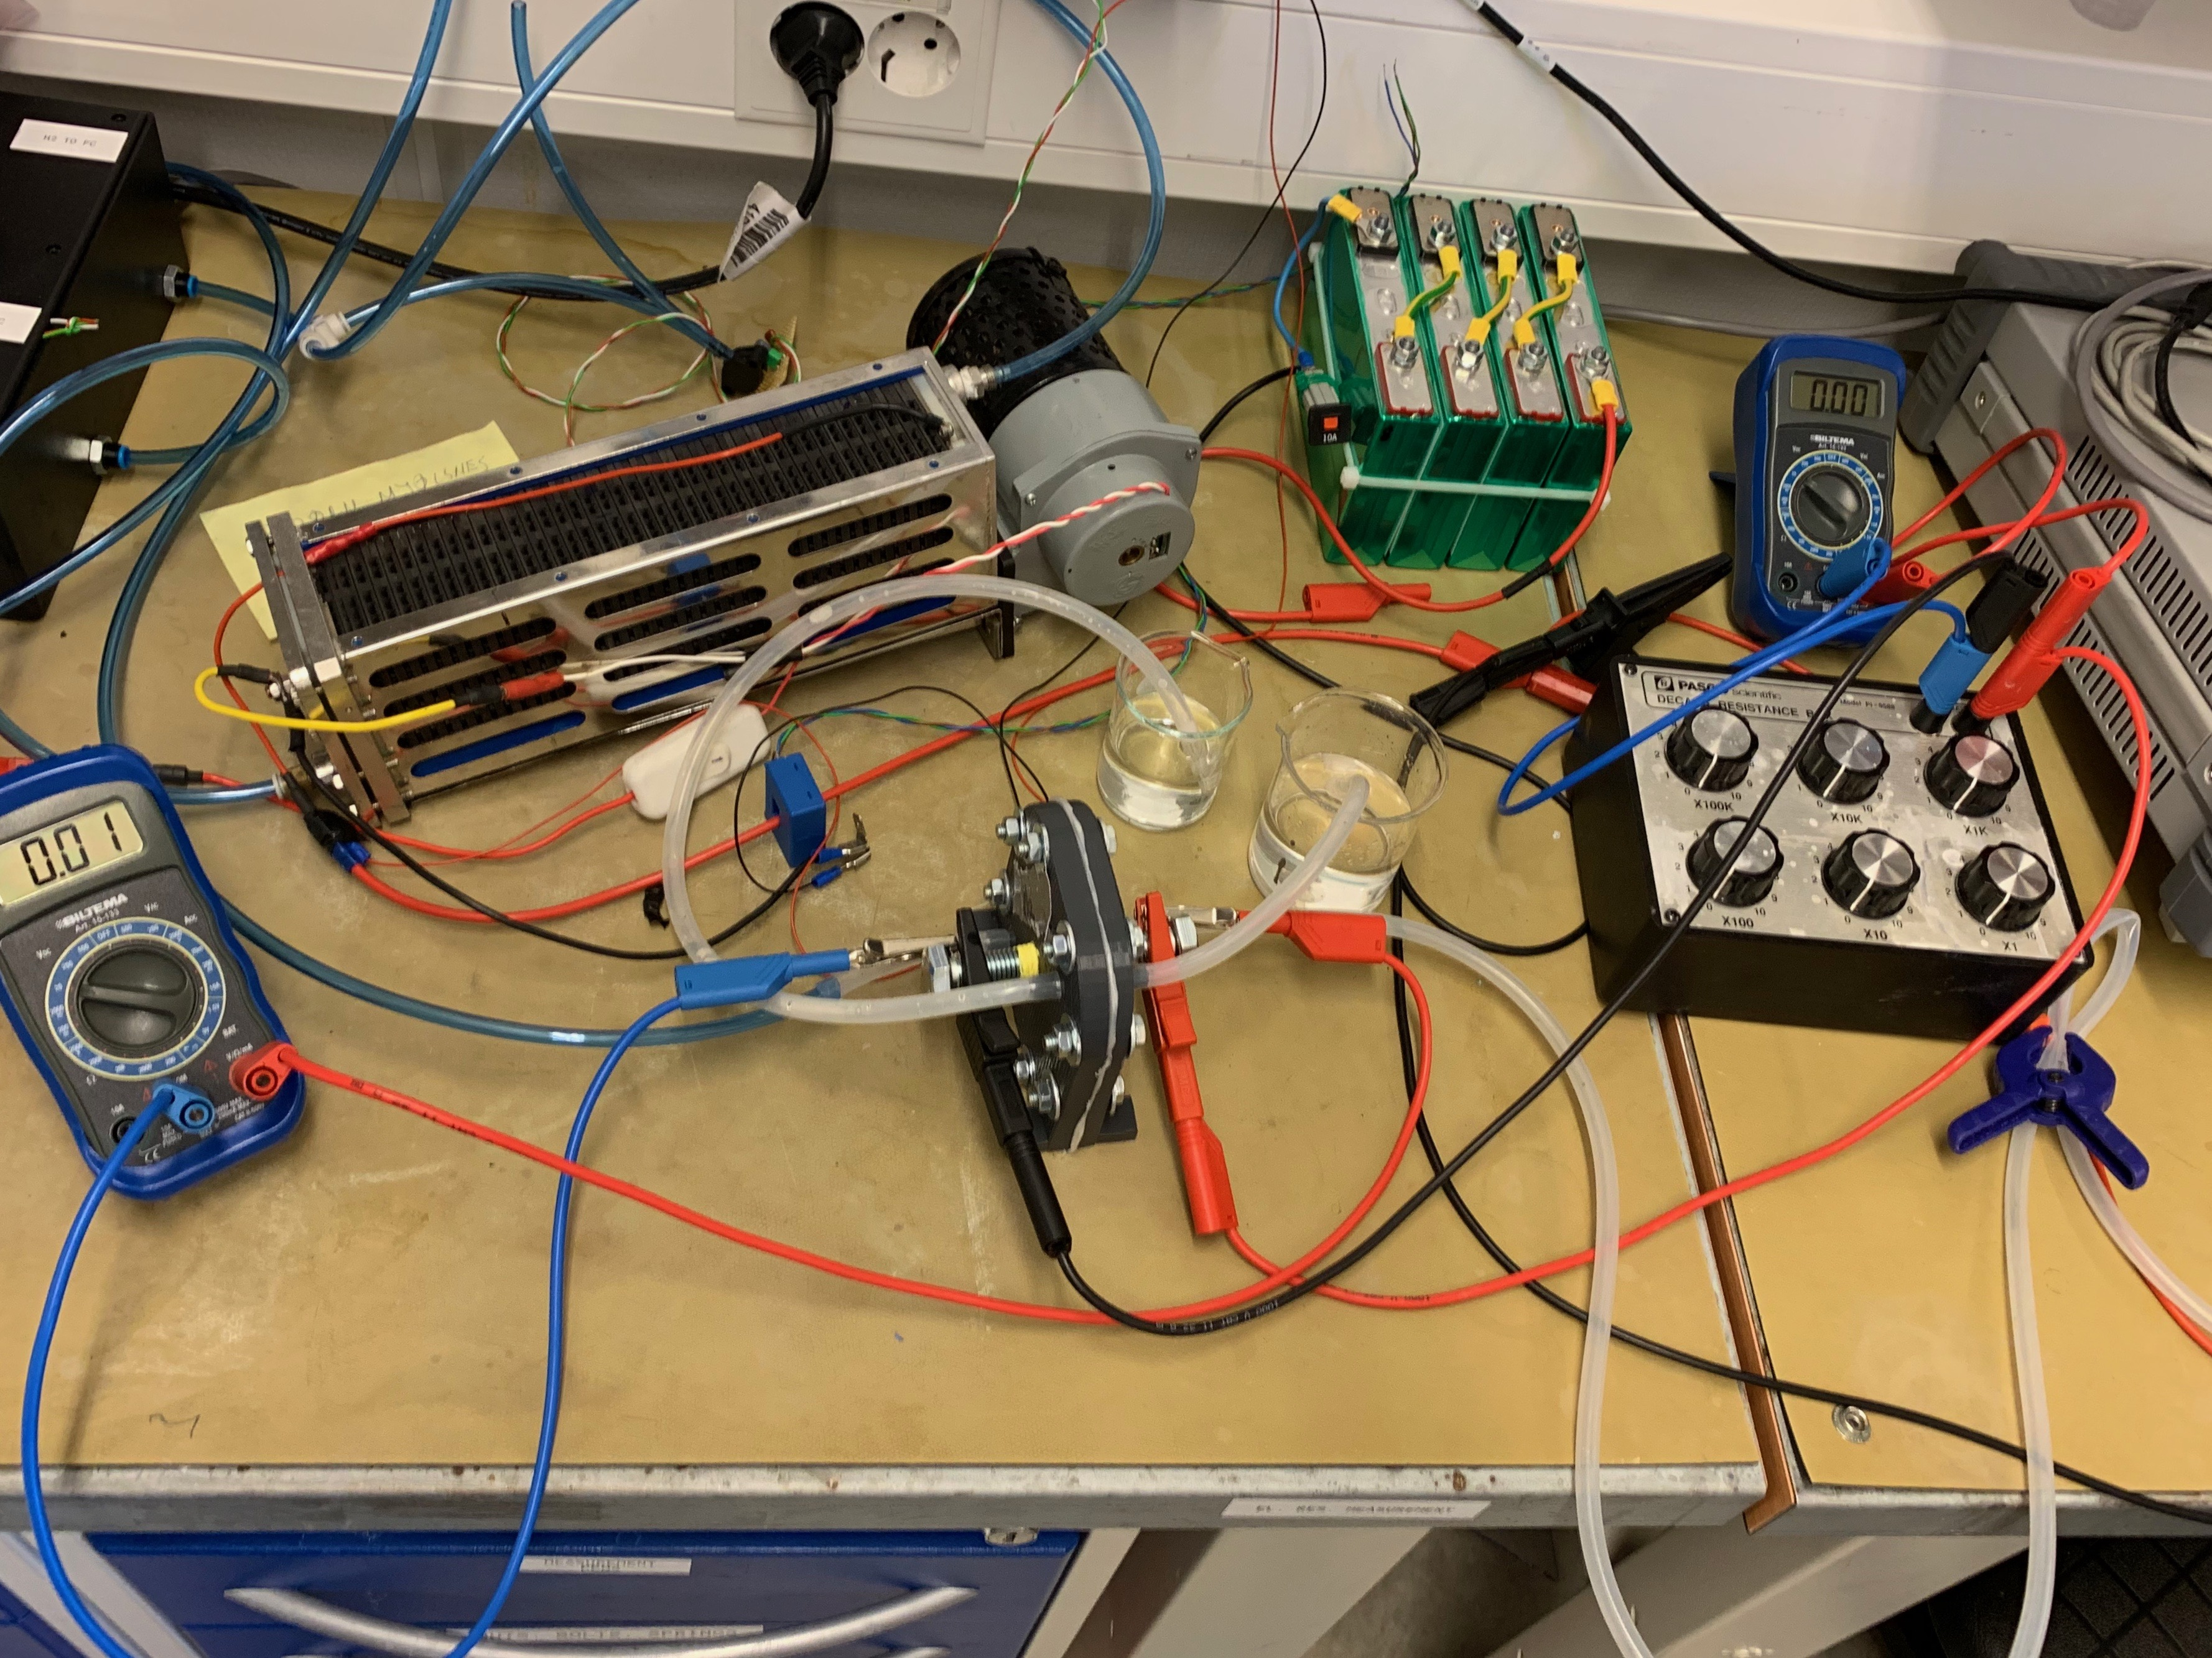
\includegraphics[width=\textwidth]{DIV./Bilder/lab.jpg}
    \caption{Test setup}
    \label{fig:TestSetup}
\end{figure}

    
\chapter{Results on ...}
    

\begin{figure}[ht]
    \centering
    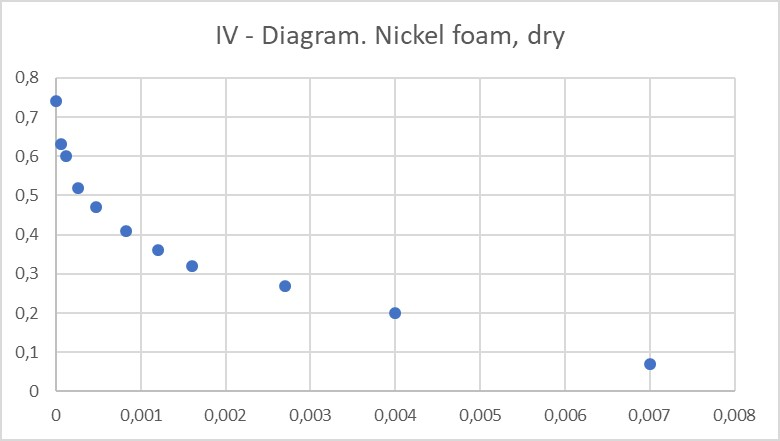
\includegraphics[width=\textwidth]{DIV./Bilder/IVcurveNFD.jpg}
    \caption{caption}
    \label{fig:IVcurveNFD}
\end{figure}

\begin{figure}[ht]
    \centering
    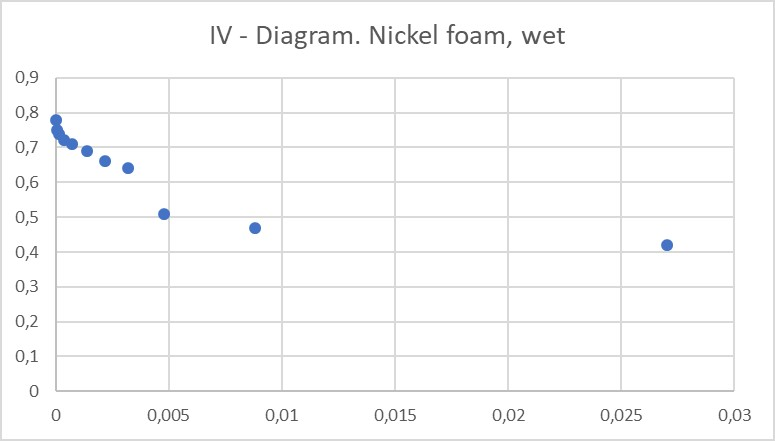
\includegraphics[width=\textwidth]{DIV./Bilder/IVcurveNFW.jpg}
    \caption{Caption}
    \label{fig:IVcurveNFW}
\end{figure}

\begin{figure}[ht]
    \centering
    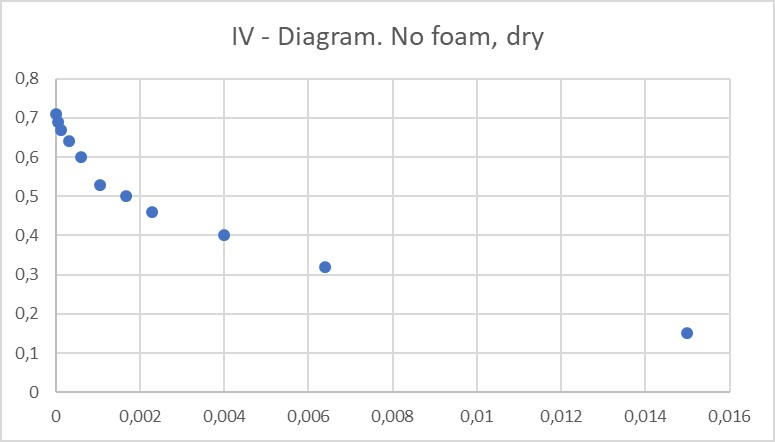
\includegraphics[width=\textwidth]{DIV./Bilder/IVcurveD.jpg}
    \caption{Caption}
    \label{fig:IVcurveD}
\end{figure}

\begin{figure}[ht]
    \centering
    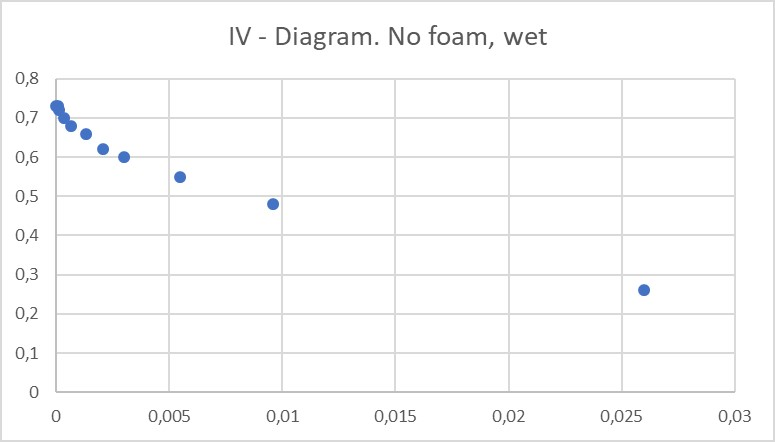
\includegraphics[width=\textwidth]{DIV./Bilder/IVcurveW.jpg}
    \caption{Caption}
    \label{fig:IVcurveW}
\end{figure}




\chapter{Discussions}
    \section{Gas diffusion}

There are many ways of diffusing the gases inside a fuel cell. One way is designing the housing whit etched channels 
to lead the gasses around in the fuel cell. The etched channels are the made to create a long way between the input and output. This way the gas gets distributed across a large part of the membrane before leaving the fuel cell. 

Another way to diffuse the gas is by using a gas diffusing layer. In our PEMFC we used a nickel foam layer to force the gas molecules to spread evenly on the membrane. 

\subsection{Etched channels for gas distribution}

We decided

By creating a distribution pattern in the fuel cell housing unit itself and making holes in the current collectors gas could be distributed to cover the whole area of the electrolyte. To save time during the modeling of the housing parts we decided to use nickel foam as a gas distribution layer, thereby making distribution patterns unnecessary.

\subsection{Flattening nickle foam}

To make the nickel foam fit inside the camper of the PEMFC it had to be flattened. To flatten it we used a hammer and a hard surface. The nickle foam is meant to distribute gas from the supply tap to cover the whole area of the electrolyte. By flattening the nickel foam there is a possibility of decreasing 

By flattening the foam we are decreasing its ability to distribute gas. This could have a effect on the results.  

\subsection{Distribution layer}

Testing shows us that we get a higher voltages while using the nickle foam for gas distribution rather then not. We believe this is because of the carbon paper does not distribute gas enough to cover the whole area of the electrolyte.    

\section{Fuel flow}
\subsection{Cross sectional supply taps}

By creating the two housing units with with "crossed patterned supply taps ??" gas would be supplied at...

\subsection{Gas flow control}

Using a manual supply valve to control the flow of hydrogen with no means to measure a flow of gas in the system there is also no way of accurately controlling that we supplied the same amount of gas flow in each test. By not supplying the same amount of hydrogen in each of the tests there might be either more or less reactions happening, giving different voltage output. There is also no way of telling that the air-pump, which is an aquarium pump, will deliver the same amount of flow at any given time. This might also cause the same concerns as expressed for hydrogen flow.

\section{Moisture management}
\subsection{Electrolyte moisture}
Testing shows us that the fuel cell performs better while the electrolyte is moist over that it does when it is dry. But we have no way of telling if water covers the whole electrolyte when we fill it with water, and if the "level of moisture" is the same in each of the wet tests and each of the dry tests...

\subsection{Damage when drying electrolyte ??}






%   Skriv diskusjonen

%   Spredningen i målinger (ohmic loss)
%   Input/output tapper kunne vært motsatt av hverandre, kunne det vært bedre?
%   Feilkilder som;
%            hvergang
%       Akvariepumpe - nøyaktig?
%       Membran kan bli dårlig av tørking gjentatte ganger?
%       Fuktighet på membranen ved ulike tester

\chapter{Conclusions}

\nocite{*}

\begin{appendix}
    \chapter{Housing drawing}
        %%%%%% DETTE TOK URIMELIG MYE TID, SÅ IKKE RØR =D - EH %%%%%%%%
\newgeometry{top=4mm, bottom=0mm, right=0mm, left=0mm}

    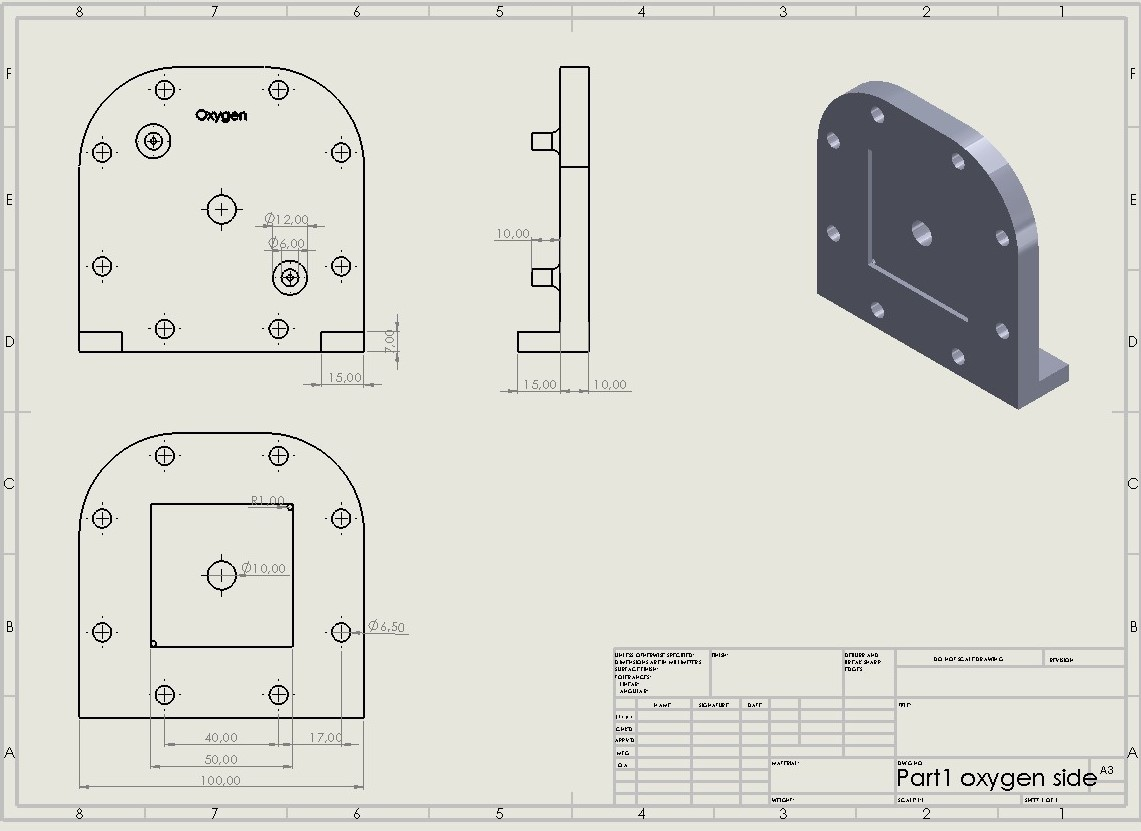
\includegraphics[angle=90,width=\textwidth,height=\textheight,keepaspectratio]{DIV./Bilder/HousingDrawing.jpg}

\restoregeometry

    \chapter{Tables}
        \section{Fuel cell with nickel foam, dry membrane}

\begin{center}
\begin{table}[h]
    \centering
        \begin{tabular}{|c|c|c|c|}
            \hline
            Resistance [\textohm] & Voltage, Fuel cell [V] & Voltage, Load [V] & Current [I] \\
            \hline
            OCV & 0.74 & 0.74 & 0 \\
            \hline
            10000 & 0.63 & 0.63 & $6.3 \times 10^{-5}$ \\
            \hline
            5000 & 0.60 & 0.60 & $1.2 \times 10^{-4}$ \\
            \hline
            2000 & 0.52 & 0.52 & $2.6 \times 10^{-4}$ \\
            \hline
            1000 & 0.47 & 0.47 & $4.7 \times 10^{-4}$ \\
            \hline
            500 & 0.41 & 0.41 & $8.2 \times 10^{-4}$ \\
            \hline
            300 & 0.36 & 0.36 & $1.2 \times 10^{-3}$ \\
            \hline
            200 & 0.32 & 0.32 & $1.6 \times 10^{-3}$ \\
            \hline
            100 & 0.27 & 0.27 & $2.7 \times 10^{-3}$ \\
            \hline
            50 & 0.20 & 0.20 & $4 \times 10^{-3}$ \\
            \hline
            10 & 0.07 & 0.07 & $7 \times 10^{-4}$ \\
            \hline
        \end{tabular}
    \caption{Fuel cell with nickel foam, Dry membrane}
    \label{tab:NickelFoamDry}
\end{table}
\end{center}

\newpage %%% ER DETTE BESTE LØSNING ???%%%%%%

\section{Fuel cell with nickel foam, wet membrane}

\begin{center}
    \begin{table}[ht]
        \centering
            \begin{tabular}{|c|c|c|c|}
            \hline
            Resistance [\textohm] & Voltage, Fuel cell [V] & Voltage, Load [V] & Current [I] \\
            \hline
            OCV & 0.78 & 0.78 & 0 \\
            \hline
            10000 & 0.75 & 0.75 & $7.5 \times 10^{-5}$ \\
            \hline
            5000 & 0.74 & 0.74 & $1.48 \times 10^{-4}$ \\
            \hline
            2000 & 0.72 & 0.72 & $3.6 \times 10^{-4}$ \\
            \hline
            1000 & 0.71 & 0.71 & $7.1 \times 10^{-4}$ \\
            \hline
            500 & 0.69 & 0.69 & $1.38 \times 10^{-3}$ \\
            \hline
            300 & 0.66 & 0.66 & $2.2 \times 10^{-3}$ \\
            \hline
            200 & 0.64 & 0.64 & $3.2 \times 10^{-3}$ \\
            \hline
            100 & 0.48 & 0.48 & $4.8 \times 10^{-3}$ \\
            \hline
            50 & 0.44 & 0.44 & $8.8 \times 10^{-3}$ \\
            \hline
            10 & 0.27 & 0.27 & $2.7 \times 10^{-2}$ \\
            \hline
        \end{tabular}
        \caption{Fuel cell with nickel foam, wet membrane}
        \label{tab:NickelFoamWet}
    \end{table}
\end{center}

\section{Fuel cell without nickel foam, dry membrane}

\begin{center}
    \begin{table}[ht]
        \centering
        \begin{tabular}{|c|c|c|c|}
            \hline
            Resistance [\textohm] & Voltage, Fuel cell [V] & Voltage, Load [V] & Current [I] \\
            \hline
            OCV & 0.71 & 0.71 & 0 \\
            \hline
            10000 & 0.69 & 0.69 & $6.9 \times 10^{-5}$ \\
            \hline
            5000 & 0.67 & 0.67 & $1.34 \times 10^{-4}$ \\
            \hline
            2000 & 0.69 & 0.69 & $3.45 \times 10^{-4}$ \\
            \hline
            1000 & 0.60 & 0.60 & $6.0 \times 10^{-4}$ \\
            \hline
            500 & 0.53 & 0.53 & $1.06 \times 10^{-3}$ \\
            \hline
            300 & 0.50 & 0.50 & $1.67 \times 10^{-3}$ \\
            \hline
            200 & 0.46 & 0.46 & $2.3 \times 10^{-3}$ \\
            \hline
            100 & 0.40 & 0.40 & $4.0 \times 10^{-3}$ \\
            \hline
            50 & 0.32 & 0.32 & $6.4 \times 10^{-3}$ \\
            \hline
            10 & 0.15 & 0.15 & $1.5 \times 10^{-2}$ \\
            \hline
        \end{tabular}
        \caption{Fuel cell without nickel foam, dry membrane}
        \label{tab:NoFoamDry}
    \end{table}
\end{center}

\newpage %%% ER DETTE BESTE LØSNING ???%%%%%%

\section{Fuel cell without nickel foam, wet membrane}

\begin{center}
    \begin{table}[ht]
        \centering
        \begin{tabular}{|c|c|c|c|}
            \hline
            Resistance [\textohm] & Voltage, Fuel cell [V] & Voltage, Load [V] & Current [I] \\
            \hline
            OCV & 0.73 & 0.73 & 0 \\
            \hline
            10000 & 0.73 & 0.73 & $7.3 \times 10^{-5}$ \\
            \hline
            5000 & 0.72 & 0.72 & $1.44 \times 10^{-4}$ \\
            \hline
            2000 & 0.70 & 0.70 & $3.5 \times 10^{-4}$ \\
            \hline
            1000 & 0.68 & 0.68 & $6.8 \times 10^{-4}$ \\
            \hline
            500 & 0.66 & 0.66 & $1.32 \times 10^{-3}$ \\
            \hline
            300 & 0.62 & 0.62 & $2.07 \times 10^{-3}$ \\
            \hline
            200 & 0.60 & 0.60 & $3.0 \times 10^{-3}$ \\
            \hline
            100 & 0.55 & 0.55 & $5.5 \times 10^{-3}$ \\
            \hline
            50 & 0.48 & 0.48 & $9.6 \times 10^{-3}$ \\
            \hline
            10 & 0.26 & 0.26 & $2.6 \times 10^{-2}$ \\
            \hline
        \end{tabular}
        \caption{Fuel cell without nickel foam, wet membrane}
        \label{tab:NoFoamWet}
    \end{table}
\end{center}
        
    \chapter{3D Printers}
        

\begin{figure}[ht]
    \centering
    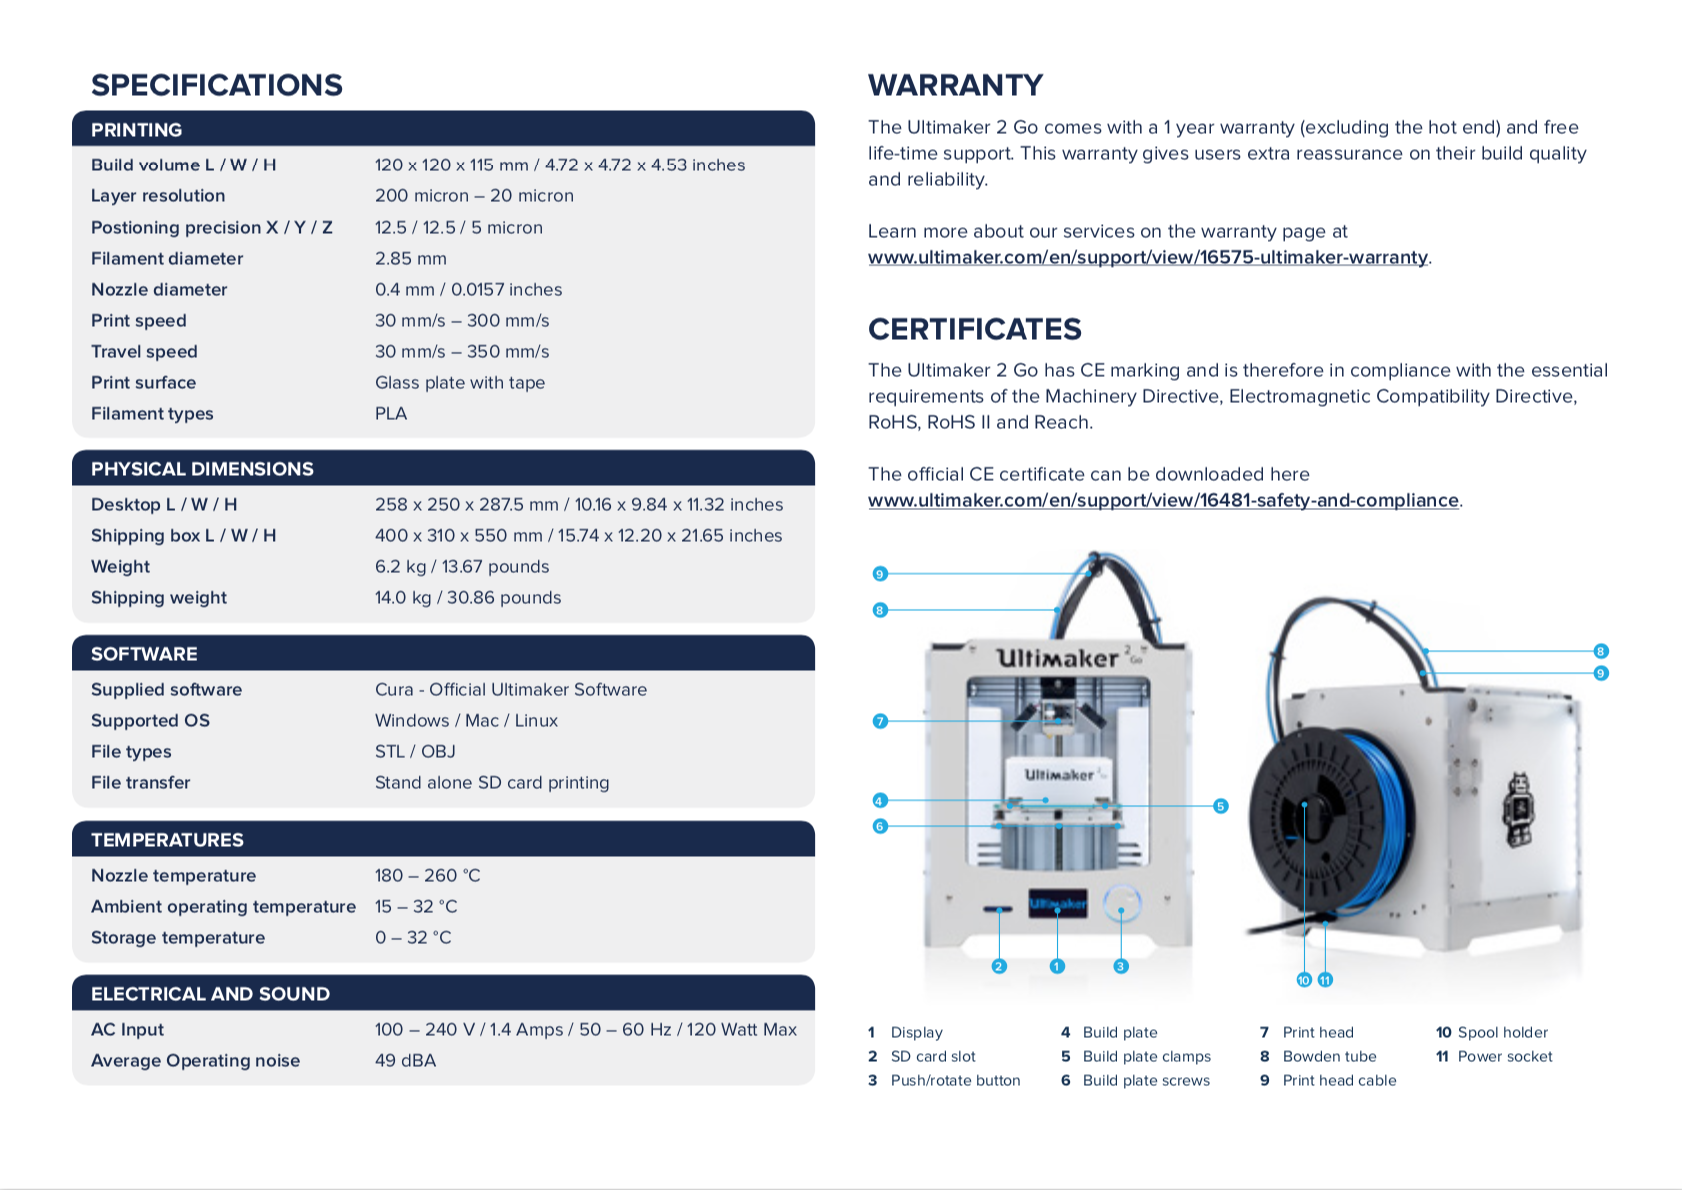
\includegraphics[angle=90, width=0.9\textwidth,]{DIV./Dokumenter/UM2Go.jpg}
\end{figure}

\begin{figure}[ht]
    \centering
    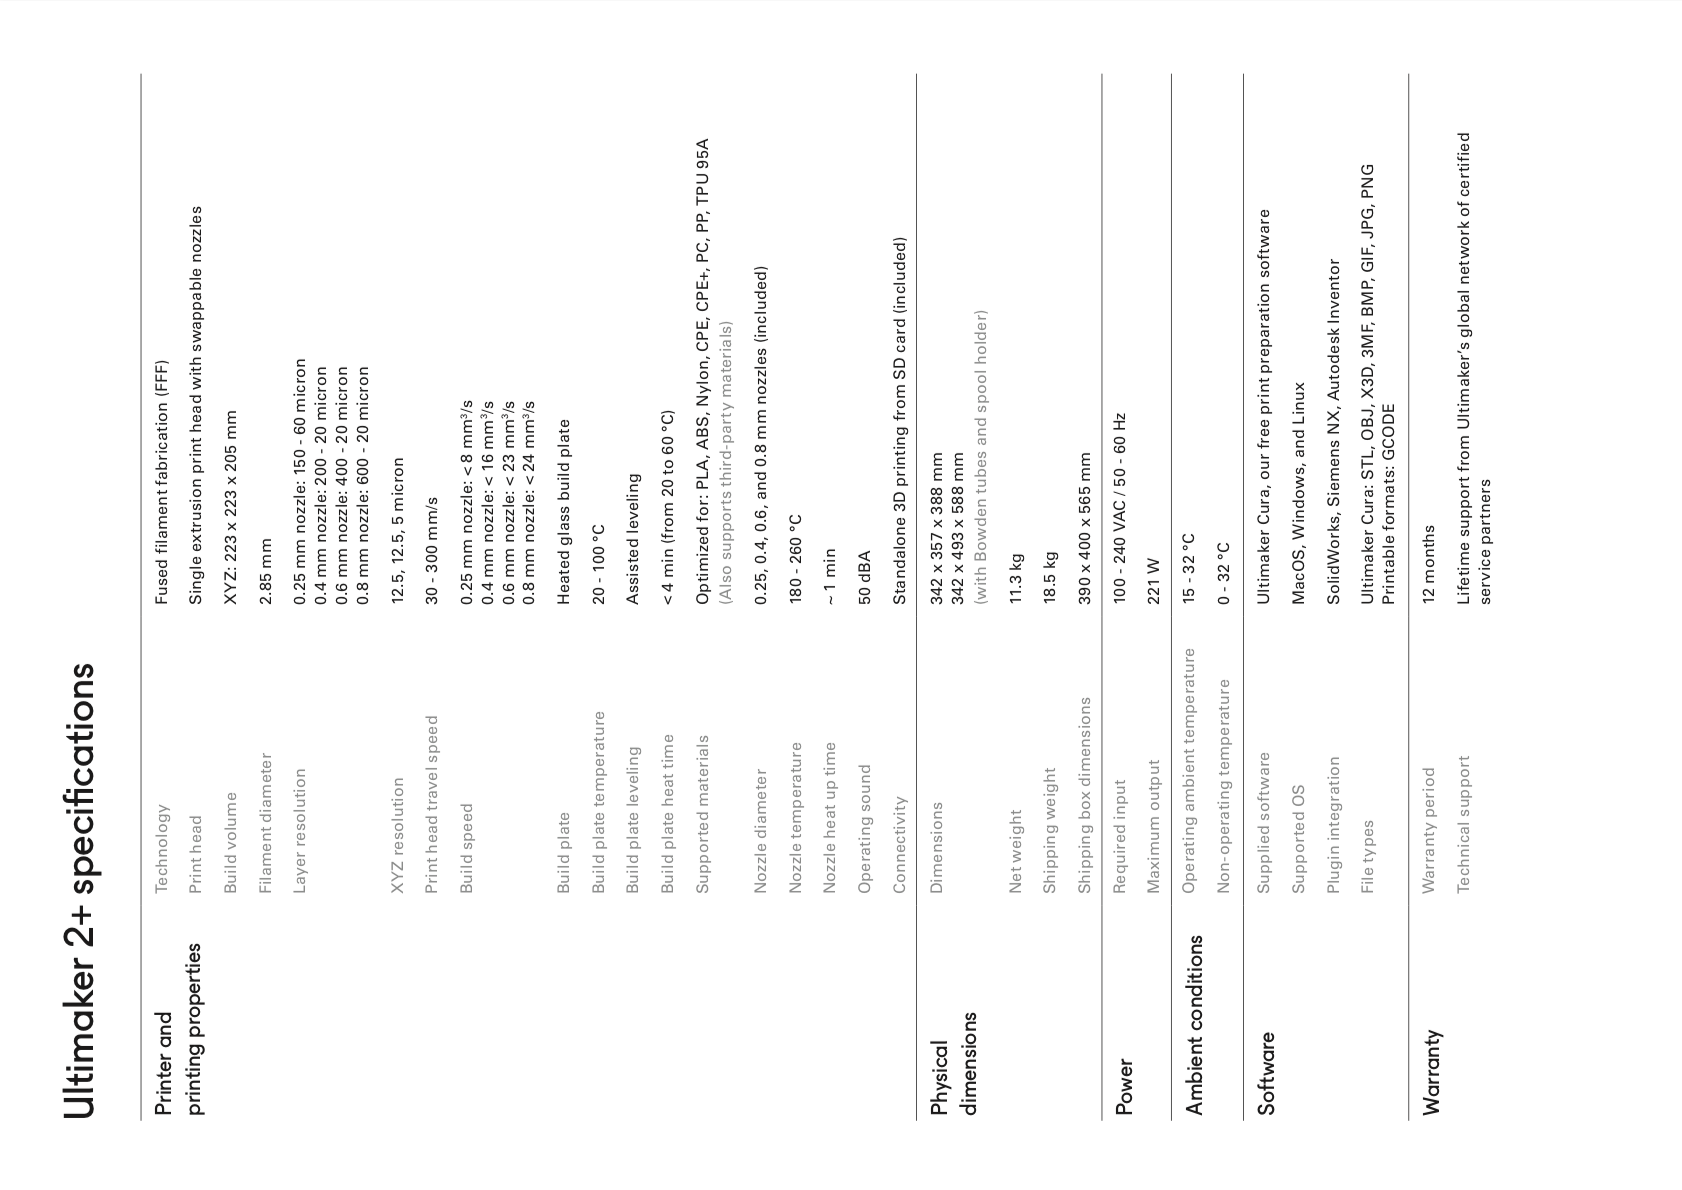
\includegraphics[angle=-90, width=0.9\textwidth]{DIV./Dokumenter/UM2+.jpg}
\end{figure}

        
    \chapter{PLA filament}
        \begin{figure}[ht]
    \centering
    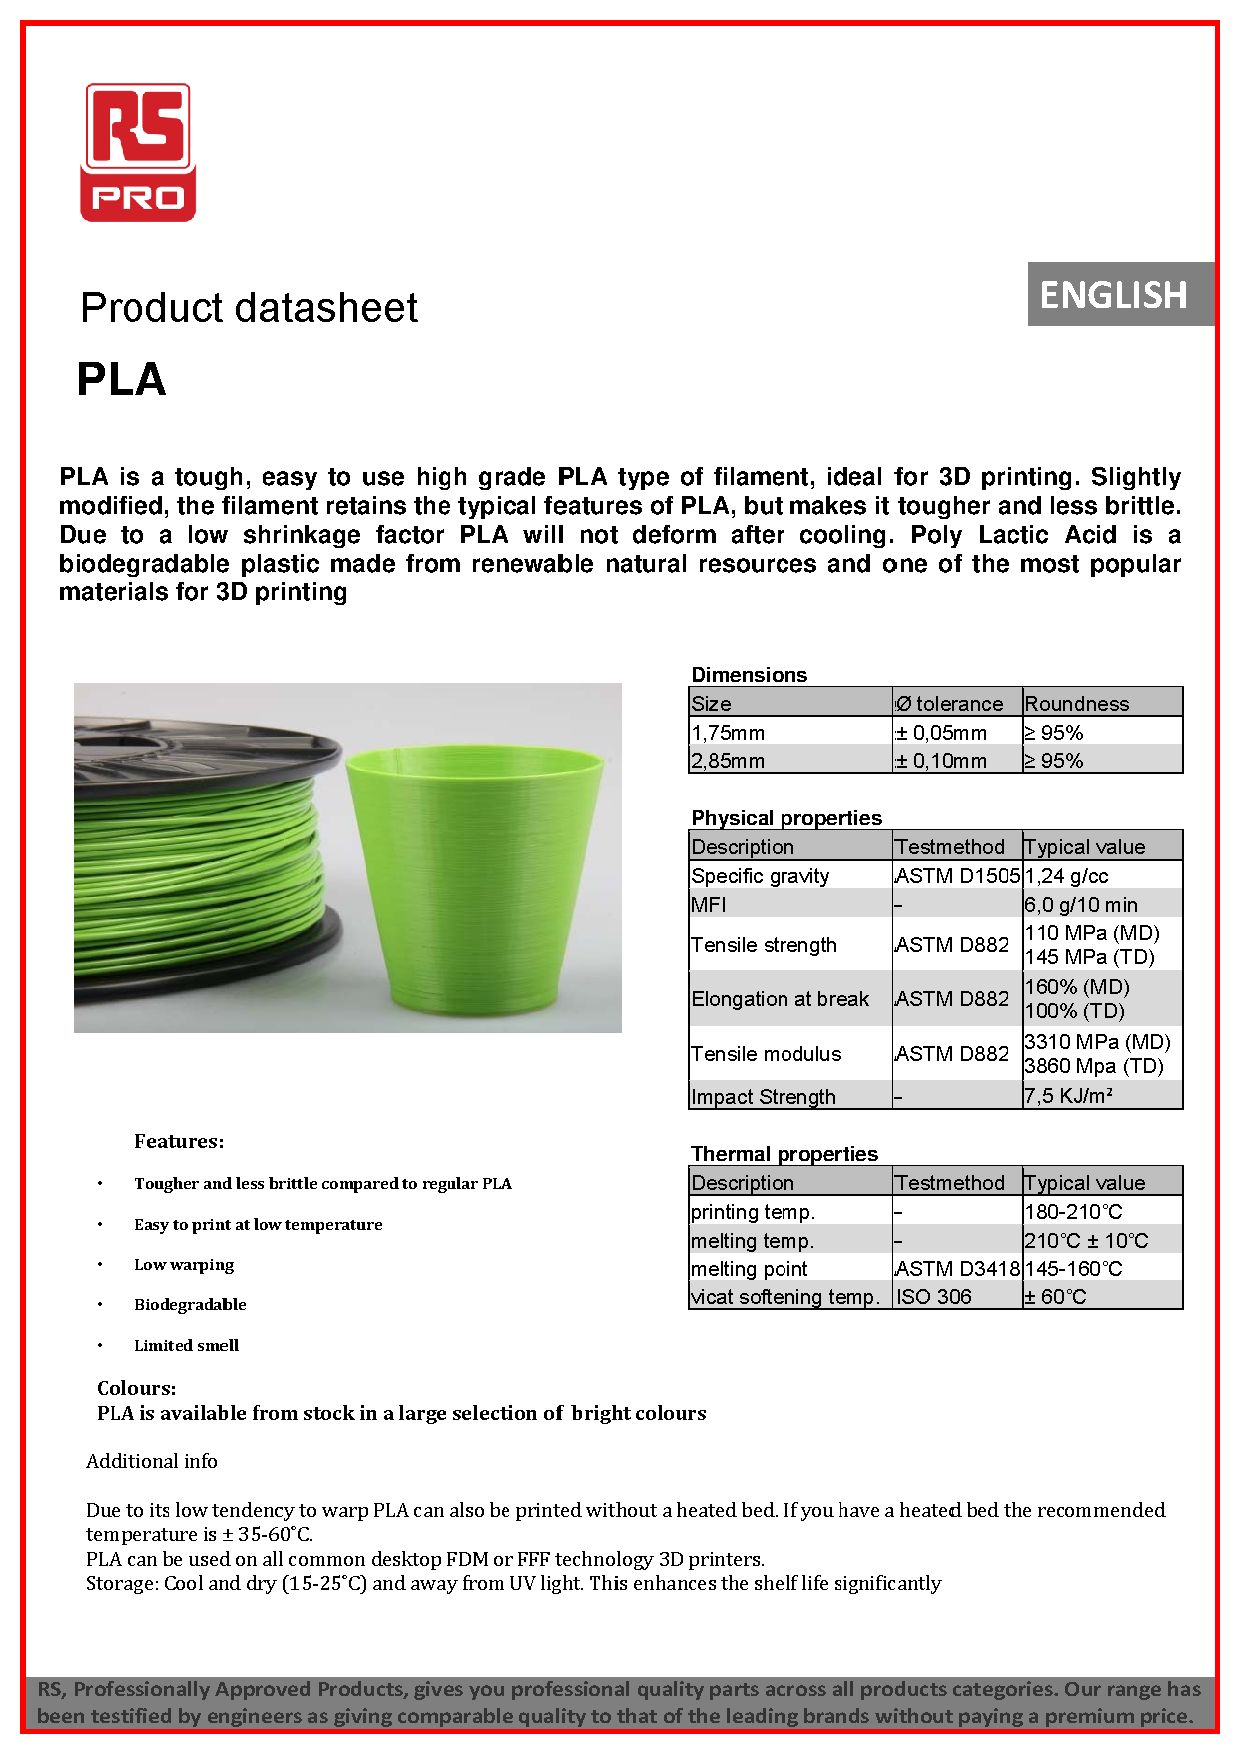
\includegraphics[width=0.9\textwidth,]{DIV./Dokumenter/PLAdok.pdf}
\end{figure}
        
\end{appendix}

\printbibliography[
heading=bibintoc,
title={Bibliography}
]


\end{document}

